%  A simple AAU report template.
%  2013-03-06 v. 1.0.0
%  Copyright 2010-2013 by Jesper Kjær Nielsen <jkn@es.aau.dk>
%
%  This is free software: you can redistribute it and/or modify
%  it under the terms of the GNU General Public License as published by
%  the Free Software Foundation, either version 3 of the License, or
%  (at your option) any later version.
%
%  This is distributed in the hope that it will be useful,
%  but WITHOUT ANY WARRANTY; without even the implied warranty of
%  MERCHANTABILITY or FITNESS FOR A PARTICULAR PURPOSE.  See the
%  GNU General Public License for more details.
%
%  You can find the GNU General Public License at <http://www.gnu.org/licenses/>.
%
%  A simple AAU report template.
%  2013-03-06 v. 1.0.0
%  Copyright 2010-2013 by Jesper Kjær Nielsen <jkn@es.aau.dk>
%
%  This is free software: you can redistribute it and/or modify
%  it under the terms of the GNU General Public License as published by
%  the Free Software Foundation, either version 3 of the License, or
%  (at your option) any later version.
%
%  This is distributed in the hope that it will be useful,
%  but WITHOUT ANY WARRANTY; without even the implied warranty of
%  MERCHANTABILITY or FITNESS FOR A PARTICULAR PURPOSE.  See the
%  GNU General Public License for more details.
%
%  You can find the GNU General Public License at <http://www.gnu.org/licenses/>.
%
\documentclass[11pt,twoside,a4paper,openright]{report}
\setcounter{tocdepth}{1}
%%%%%%%%%%%%%%%%%%%%%%%%%%%%%%%%%%%%%%%%%%%%%%%%
% Language, Encoding and Fonts
% http://en.wikibooks.org/wiki/LaTeX/Internationalization
%%%%%%%%%%%%%%%%%%%%%%%%%%%%%%%%%%%%%%%%%%%%%%%%
% Select encoding of your inputs. Depends on
% your operating system and its default input
% encoding. Typically, you should use
%   Linux  : utf8 (most modern Linux distributions)
%            latin1 
%   Windows: ansinew
%            latin1 (works in most cases)
%   Mac    : applemac
% Notice that you can manually change the input
% encoding of your files by selecting "save as"
% an select the desired input encoding. 
\usepackage[utf8]{inputenc}
% Make latex understand and use the typographic
% rules of the language used in the document.
\usepackage[danish,english]{babel}
% Use the vector font Latin Modern which is going
% to be the default font in latex in the future.
\usepackage{lmodern}
% Choose the font encoding
\usepackage[T1]{fontenc}
%%%%%%%%%%%%%%%%%%%%%%%%%%%%%%%%%%%%%%%%%%%%%%%%
% Graphics and Tables
% http://en.wikibooks.org/wiki/LaTeX/Importing_Graphics
% http://en.wikibooks.org/wiki/LaTeX/Tables
% http://en.wikibooks.org/wiki/LaTeX/Colors
%%%%%%%%%%%%%%%%%%%%%%%%%%%%%%%%%%%%%%%%%%%%%%%%
% load a colour package
\usepackage{xcolor}
\usepackage{longtable}
\definecolor{aaublue}{RGB}{33,26,82}% dark blue
% The standard graphics inclusion package
\usepackage{graphicx}
% Set up how figure and table captions are displayed
\usepackage{caption}
\captionsetup{%
  font=footnotesize,% set font size to footnotesize
  labelfont=bf % bold label (e.g., Figure 3.2) font
}
% Make the standard latex tables look so much better
\usepackage{array,booktabs}
% Enable the use of frames around, e.g., theorems
% The framed package is used in the example environment
\usepackage{framed}


%%%%%%%%%%%%%%%%%%%%%%%%%%%%%%%%%%%%%%%%%%%%%%%%
% Mathematics
% http://en.wikibooks.org/wiki/LaTeX/Mathematics
%%%%%%%%%%%%%%%%%%%%%%%%%%%%%%%%%%%%%%%%%%%%%%%%
% Defines new environments such as equation,
% align and split 
\usepackage{amsmath}
% Adds new math symbols
\usepackage{amssymb}
% Use theorems in your document
% The ntheorem package is also used for the example environment
% When using thmmarks, amsmath must be an option as well. Otherwise \eqref doesn't work anymore.
\usepackage[framed,amsmath,thmmarks]{ntheorem}

%%%%%%%%%%%%%%%%%%%%%%%%%%%%%%%%%%%%%%%%%%%%%%%%
% Page Layout
% http://en.wikibooks.org/wiki/LaTeX/Page_Layout
%%%%%%%%%%%%%%%%%%%%%%%%%%%%%%%%%%%%%%%%%%%%%%%%
% Change margins, papersize, etc of the document
\usepackage[
  left=28mm,% left margin on an odd page
  right=41mm,% right margin on an odd page
  ]{geometry}
% Modify how \chapter, \section, etc. look
% The titlesec package is very configureable
\usepackage{titlesec}
\titleformat*{\section}{\normalfont\Large\bfseries\color{aaublue}}
\titleformat*{\subsection}{\normalfont\large\bfseries\color{aaublue}}
\titleformat*{\subsubsection}{\normalfont\normalsize\bfseries\color{aaublue}}
%\titleformat*{\paragraph}{\normalfont\normalsize\bfseries\color{aaublue}}
%\titleformat*{\subparagraph}{\normalfont\normalsize\bfseries\color{aaublue}}

% Change the headers and footers
\usepackage{fancyhdr}
\pagestyle{fancy}
\fancyhf{} %delete everything
\renewcommand{\headrulewidth}{0pt} %remove the horizontal line in the header
\fancyhead[RE]{\color{aaublue}\small\nouppercase\leftmark} %even page - chapter title
\fancyhead[LO]{\color{aaublue}\small\nouppercase\rightmark} %uneven page - section title
\fancyhead[LE,RO]{\thepage} %page number on all pages
% Do not stretch the content of a page. Instead,
% insert white space at the bottom of the page
\raggedbottom
% Enable arithmetics with length. Useful when
% typesetting the layout.
\usepackage{calc}
\usepackage{graphicx}
\graphicspath{ {./figures/}{./figures/prototype-comp/} }
\usepackage{subcaption}
%%%%%%%%%%%%%%%%%%%%%%%%%%%%%%%%%%%%%%%%%%%%%%%%
% Bibliography
% http://en.wikibooks.org/wiki/LaTeX/Bibliography_Management
%%%%%%%%%%%%%%%%%%%%%%%%%%%%%%%%%%%%%%%%%%%%%%%%
% Add the \citep{key} command which display a
% reference as [author, year]
\usepackage[backend=bibtex,
  bibencoding=utf8
  ]{biblatex}
\addbibresource{bib/mybib}
%\usepackage[square]{natbib}
% Appearance of the bibliography
%\bibliographystyle{apalike}
\usepackage{csquotes}
\renewcommand{\mkbegdispquote}[2]{\itshape}
%%%%%%%%%%%%%%%%%%%%%%%%%%%%%%%%%%%%%%%%%%%%%%%%
% Misc
%%%%%%%%%%%%%%%%%%%%%%%%%%%%%%%%%%%%%%%%%%%%%%%%
% Add bibliography and index to the table of
% contents
\usepackage[nottoc]{tocbibind}
% Add the command \pageref{LastPage} which refers to the
% page number of the last page
\usepackage[
%  disable, %turn off todonotes
  colorinlistoftodos, %enable a coloured square in the list of todos
  textwidth=\marginparwidth, %set the width of the todonotes
  textsize=scriptsize, %size of the text in the todonotes
  ]{todonotes}
% added by KK (ShareLaTeX team)
\usepackage{lastpage}

%%%%%%%%%%%%%%%%%%%%%%%%%%%%%%%%%%%%%%%%%%%%%%%%
% Hyperlinks
% http://en.wikibooks.org/wiki/LaTeX/Hyperlinks
%%%%%%%%%%%%%%%%%%%%%%%%%%%%%%%%%%%%%%%%%%%%%%%%
% Enable hyperlinks and insert info into the pdf
% file. Hypperref should be loaded as one of the 
% last packages
\usepackage{hyperref}
\hypersetup{%
%	pdfpagelabels=true,%
	plainpages=false,%
	pdfauthor={Author(s)},%
	pdftitle={Title},%
	pdfsubject={Subject},%
	bookmarksnumbered=true,%
	colorlinks,%
	citecolor=aaublue,%
	filecolor=aaublue,%
	linkcolor=aaublue,% you should probably change this to black before printing
	urlcolor=aaublue,%
	pdfstartview=FitH%
}
\usepackage{wrapfig}


% LST Listings
\definecolor{bluekeywords}{rgb}{0,0,1}
\definecolor{greencomments}{rgb}{0,0.5,0}
\definecolor{redstrings}{rgb}{0.64,0.08,0.08}
\definecolor{xmlcomments}{rgb}{0.5,0.5,0.5}
\definecolor{types}{rgb}{0.17,0.57,0.68}

\definecolor{ForrestGreen}{RGB}{0,100,0}
\usepackage{listings}
\lstset{language=C,
literate=%
{æ}{{\ae}}1
{å}{{\aa}}1
{ø}{{\o}}1
{Æ}{{\AE}}1
{Å}{{\AA}}1
{Ø}{{\O}}1,
captionpos=t,
frame=lines,
numbers=left,
stepnumber=1,
showspaces=false,
showtabs=false,
breaklines=true,
showstringspaces=false,
breakatwhitespace=true,
escapeinside={(*@}{@*)},
commentstyle=\color{greencomments},
morecomment=[l]{\# },
keywordstyle=\color{bluekeywords},
emph={class, true, false, public, private, override, Time, Input, Random, KeyCode, Debug, using, StreamReader, Path, Environment, new, Length, OrderBy, ToArray, Count, Range, ExecuteNonQuery, Parameters, SqlCommand, AddWithValue},          
emphstyle=\ttfamily\color{ForrestGreen}, 
morekeywords={partial,var,value,class},
stringstyle=\color{redstrings},
basicstyle=\ttfamily\small,
classoffset=1, % starting new class
morekeywords={bool, boolean, float, double, Vector1, Vector2, Vector3, string, char, var, foreach, try, finally, Math, text, number, catch},
otherkeywords={bool, boolean, float, double, Vector1, Vector2, Vector3, string, char, var, foreach, try, finally, Math, text, number, catch},
keywordstyle=\color{bluekeywords},
classoffset=0,
}

\usepackage[normalem]{ulem}
\useunder{\uline}{\ul}{}

\usepackage{booktabs}
\usepackage{lscape}

% Command to rotate a text -90 degrees.
\newcommand*\rot{\rotatebox{-90}}

\usepackage{float}

\usepackage{pdfpages}

\usepackage{tikz}
\usetikzlibrary{calc,trees,positioning,arrows,chains,shapes.geometric,%
    decorations.pathreplacing,decorations.pathmorphing,shapes,%
    matrix,shapes.symbols}
    
\tikzset{
>=stealth',
  punktchain/.style={
    rectangle, 
    rounded corners, 
    % fill=black!10,
    draw=black, very thick,
    text width=10em, 
    minimum height=3em, 
    text centered, 
    on chain},
  line/.style={draw, thick, <-},
  element/.style={
    tape,
    top color=white,
    bottom color=blue!50!black!60!,
    minimum width=8em,
    draw=blue!40!black!90, very thick,
    text width=10em, 
    minimum height=3.5em, 
    text centered, 
    on chain},
  every join/.style={->, thick,shorten >=1pt},
  decoration={brace},
  tuborg/.style={decorate},
  tubnode/.style={midway, right=2pt},
}

\usepackage{mathtools}

\usepackage{graphicx}
\graphicspath{ {./figures/}{./figures/prototype-comp/} }
\usepackage{subcaption}
\usepackage{listings}% package inclusion and set up of the document
% see, e.g., http://en.wikibooks.org/wiki/LaTeX/Formatting#Hyphenation
% for more information on word hyphenation
\hyphenation{ex-am-ple hy-phen-a-tion short}
\hyphenation{long la-tex}
% 
%  A simple AAU report template.
%  2013-03-06 v. 1.0.0
%  Copyright 2010-2013 by Jesper Kjær Nielsen <jkn@es.aau.dk>
%
%  This is free software: you can redistribute it and/or modify
%  it under the terms of the GNU General Public License as published by
%  the Free Software Foundation, either version 3 of the License, or
%  (at your option) any later version.
%
%  This is distributed in the hope that it will be useful,
%  but WITHOUT ANY WARRANTY; without even the implied warranty of
%  MERCHANTABILITY or FITNESS FOR A PARTICULAR PURPOSE.  See the
%  GNU General Public License for more details.
%
%  You can find the GNU General Public License at <http://www.gnu.org/licenses/>.
%
%
%
% see, e.g., http://en.wikibooks.org/wiki/LaTeX/Customizing_LaTeX#New_commands
% for more information on how to create macros

%%%%%%%%%%%%%%%%%%%%%%%%%%%%%%%%%%%%%%%%%%%%%%%%
% Macros for the titlepage
%%%%%%%%%%%%%%%%%%%%%%%%%%%%%%%%%%%%%%%%%%%%%%%%
%Creates the aau titlepage
\newcommand{\aautitlepage}[3]{%
  {
    %set up various length
    \ifx\titlepageleftcolumnwidth\undefined
      \newlength{\titlepageleftcolumnwidth}
      \newlength{\titlepagerightcolumnwidth}
    \fi
    \setlength{\titlepageleftcolumnwidth}{0.5\textwidth-\tabcolsep}
    \setlength{\titlepagerightcolumnwidth}{\textwidth-2\tabcolsep-\titlepageleftcolumnwidth}
    %create title page
    \thispagestyle{empty}
    \noindent%
    \begin{tabular}{@{}ll@{}}
      \parbox{\titlepageleftcolumnwidth}{
        \iflanguage{danish}{%
          
\includegraphics[width=\titlepageleftcolumnwidth]{figures/aau_logo_da}
        }{%
          
\includegraphics[width=\titlepageleftcolumnwidth]{figures/aau_logo_en}
        }
      } &
      \parbox{\titlepagerightcolumnwidth}{\raggedleft\sf\small
        #2
      }\bigskip\\
       #1 &
      \parbox[t]{\titlepagerightcolumnwidth}{%
      \textbf{Abstract:}\bigskip\par
        \fbox{\parbox{\titlepagerightcolumnwidth-2\fboxsep-2\fboxrule}{%
          #3
        }}
      }\\
    \end{tabular}
    \vfill
    \iflanguage{danish}{%
      \noindent{\footnotesize\emph{Rapportens indhold er frit tilgængeligt, men offentliggørelse (med kildeangivelse) må kun ske efter aftale med forfatterne.}}
    }{%
      \noindent{\footnotesize\emph{The content of this report is freely available, but publication (with reference) may only be pursued due to agreement with the author.}}
    }
    \clearpage
  }
}

%Create english project info
\newcommand{\englishprojectinfo}[8]{%
  \parbox[t]{\titlepageleftcolumnwidth}{
    \textbf{Title:}\\ #1\bigskip\par
    \textbf{Theme:}\\ #2\bigskip\par
    \textbf{Project Period:}\\ #3\bigskip\par
    \textbf{Project Group:}\\ #4\bigskip\par
    \textbf{Participant(s):}\\ #5\bigskip\par
    \textbf{Supervisor(s):}\\ #6\bigskip\par
    \textbf{Copies:} #7\bigskip\par
    \textbf{Page Numbers:} \pageref{LastPage}\bigskip\par
    \textbf{Date of Completion:}\\ #8
  }
}

%Create danish project info
\newcommand{\danishprojectinfo}[8]{%
  \parbox[t]{\titlepageleftcolumnwidth}{
    \textbf{Titel:}\\ #1\bigskip\par
    \textbf{Tema:}\\ #2\bigskip\par
    \textbf{Projektperiode:}\\ #3\bigskip\par
    \textbf{Projektgruppe:}\\ #4\bigskip\par
    \textbf{Deltager(e):}\\ #5\bigskip\par
    \textbf{Vejleder(e):}\\ #6\bigskip\par
    \textbf{Oplagstal:} #7\bigskip\par
    \textbf{Sidetal:} \pageref{LastPage}\bigskip\par
    \textbf{Afleveringsdato:}\\ #8
  }
}

%%%%%%%%%%%%%%%%%%%%%%%%%%%%%%%%%%%%%%%%%%%%%%%%
% An example environment
%%%%%%%%%%%%%%%%%%%%%%%%%%%%%%%%%%%%%%%%%%%%%%%%
\theoremheaderfont{\normalfont\bfseries}
\theorembodyfont{\normalfont}
\theoremstyle{break}
\def\theoremframecommand{{\color{aaublue!50}\vrule width 5pt \hspace{5pt}}}
\newshadedtheorem{exa}{Example}[chapter]
\newenvironment{example}[1]{%
		\begin{exa}[#1]
}{%
		\end{exa}
}
% my new macros
%\titleformat{\chapter}[hang]{\normalfont\huge\bfseries}{\thechapter}{1em}{}
%\titleformat{\section}
%{\normalfont\LARGE\bfseries}{\thesection}{1em}{}
%\titleformat{\subsection}
%{\normalfont\Large\bfseries}{\thesubsection}{1em}{}
%\titleformat{\subsubsection}
%{\normalfont\large\bfseries}{\thesubsubsection}{1em}{}
%\titlespacing\chapter{0pt}{-20pt}{20pt}
%\titlespacing\section{0pt}{12pt plus 4pt minus 2pt}{-2pt plus 2pt minus 2pt}
%\titlespacing\subsection{0pt}{12pt plus 4pt minus 2pt}{-2pt plus 2pt minus 2pt}
%\titlespacing\subsubsection{0pt}{12pt plus 4pt minus 2pt}{-2pt plus 2pt minus 2pt}

\begin{document}
%frontmatter
\pagestyle{empty} %disable headers and footers
\pagenumbering{roman} %use roman page numbering in the frontmatter
%  A simple AAU report template.
%  2013-03-06 v. 1.0.0
%  Copyright 2010-2013 by Jesper Kjær Nielsen <jkn@es.aau.dk>
%
%  This is free software: you can redistribute it and/or modify
%  it under the terms of the GNU General Public License as published by
%  the Free Software Foundation, either version 3 of the License, or
%  (at your option) any later version.
%
%  This is distributed in the hope that it will be useful,
%  but WITHOUT ANY WARRANTY; without even the implied warranty of
%  MERCHANTABILITY or FITNESS FOR A PARTICULAR PURPOSE.  See the
%  GNU General Public License for more details.
%
%  You can find the GNU General Public License at <http://www.gnu.org/licenses/>.
%
\pdfbookmark[0]{Front page}{label:frontpage}%
\begin{titlepage}
  \addtolength{\hoffset}{0.5\evensidemargin-0.5\oddsidemargin} %set equal margins on the frontpage - remove this line if you want default margins
  \noindent%
  \begin{tabular}{@{}p{\textwidth}@{}}
    \toprule[2pt]
    \midrule
    \vspace{0.2cm}
    \begin{center}
    \Huge{\textbf{
      Personal Home Automation Language% insert your title here
    }}
    \end{center}
    \begin{center}
      \Large{
        - An intuitive programming language for Arduino -% insert your subtitle here
      }
    \end{center}
    \vspace{0.2cm}\\
    \midrule
    \toprule[2pt]
  \end{tabular}
  \vspace{4 cm}
  \begin{center}
    {\large
      Project Report%Insert document type (e.g., Project Report)
    }\\
    \vspace{0.2cm}
    {\Large
      Group: SW404F18%Insert your group name or real names here
    }
  \end{center}
  \vfill
  \begin{center}
  Aalborg University\\
  Department of Computer Science\\
  Selma Lagerlöfs Vej 300\\
  9220 Aalborg East, DK
  \end{center}
\end{titlepage}
\clearpage

\thispagestyle{empty}
{\small
\strut\vfill % push the content to the bottom of the page
\noindent Copyright \copyright{} Aalborg University 2018\par
\vspace{0.2cm}
\noindent Photographic, mechanic or any other form of duplication of this paper is not allowed according to Danish copyright law and without permission by the authors.
}
\clearpage


\pdfbookmark[0]{English title page}{label:titlepage_en}
\aautitlepage{%
  \englishprojectinfo{
    Product Owner of GIRAF%title
  }{%
  Prototypes, usability testing and customer contac %theme
  }{%
    Spring Semester 2019 %project period
  }{%
    SW610f19 % project group
  }{%
    %list of group members
    Andreas Stenshøj\\ 
    Daniel Moesgaard Andersen\\
    Frederik Valdemar Schrøder\\
    Jens Petur Tróndarson\\
    Rasmus Bundgaard Eduardsen\\
    Mathias Møller Lybech
  }{%
    %list of supervisors
    Chenjuan Guo\\
  }{%
    1 % number of printed copies
  }{%
    May 28, 2018 % date of completion
  }%
}{%department and address
  \textbf{Department of Computer Science}\\
  Aalborg University\\
  Selma Lagerlöfs Vej 300\\
  9220 Aalborg East, DK\\
  \href{www.cs.aau.dk}{www.cs.aau.dk}
}{% the abstract
The abstract is right here
}

%\cleardoublepage
%{\selectlanguage{danish}
%\pdfbookmark[0]{Danish title page}{label:titlepage_da}
%\aautitlepage{%
%  \danishprojectinfo{
%    Rapportens titel %title
%  }{%
%    Semestertema %theme
%  }{%
%    Efterårssemestret 2010 %project period
%  }{%
%    XXX % project group
%  }{%
%    %list of group members
%    Forfatter 1\\ 
%    Forfatter 2\\
%    Forfatter 3
%  }{%
%    %list of supervisors
%    Vejleder 1\\
%    Vejleder 2
%  }{%
%    1 % number of printed copies
%  }{%
%    \today % date of completion
%  }%
%}{%department and address
%  \textbf{Institut for Elektroniske Systemer}\\
%  Fredrik Bajers Vej 7\\
%  DK-9220 Aalborg Ø\\
%  \href{http://es.aau.dk}{http://es.aau.dk}
%}{% the abstract
%  Her er resuméet
%}}

\cleardoublepage
\pdfbookmark[0]{Contents}{label:contents}
\pagestyle{fancy} %enable headers and footers again
\tableofcontents
\cleardoublepage
%mainmatter
\pagenumbering{arabic} %use arabic page numbering in the mainmatter
\listoftodos
\chapter{Introduction}
Autism spectrum disorder (ASD) is a condition that is characterized by a broad range of challenges within different areas such as social skills, speech and nonverbal communication, or by causing repetitive behavior.
In 2014 there were 16.8 occurrences of the ASD diagnosis per 1,000 children, and approximately 1\% of all Danes have an ASD diagnosis \autocite{cdcdata}. 
As ASD is a spectrum disorder, each person diagnosed with it has different strengths and challenges.
This results in people with ASD learning, thinking and solving problems very differently, with ranges from highly skilled and functional to severely challenged. 
Some may require support in their daily lives while others on the spectrum can live entirely independently \autocite{autismspeaks}.

\section{About GIRAF}
GIRAF (Graphical Interface Resource for Autistic Folk) is an ongoing project developed by 6th semester software engineering students at Aalborg University. 
The project has been continuously developed on since 2011 with Ulrik Mathias Nyman as project coordinator, with the new students assuming responsibility and learning to cooperate in a bigger environment with an existing codebase. 
\\
GIRAF is a program that serves the purpose of helping people with autism, with the primary user group being children.
The primary goal of the system is to provide visual representation of the daily or weekly schedule for the users.
During the lifetime of the project, different types of games and communication tools to help with education have been implemented, but most of these functionalities do not work after the API rework of 2017. The current focus of the GIRAF project is to make the weekplanner stable and fit for use, before resuming work on the other parts of the project. 
\\\\
A special aspect of the project, in comparison to previous projects, is the direct interaction with real customers, who are essential for the project.
The customers serve to define requirements of the program and facilitate the familiarization of students with industry processes.
\\
\noindent
Currently the institutions that are represented are: 
\begin{itemize}
    \item Mette and Emil, Egebakken (School)
    \item Kristine and Susanne, Birken (Kindergarten)
    \item Flemming, Center for Autism
    \item Niels, IT manager in the elderly and disability administration.
\end{itemize}

\input{sections/introduction/state-of-giraf}
\section{State of Giraf}
The purpose of this section is to describe the current state of Giraf as it is delivered to us. 
This is done so that we have an idea of what our starting point will be,
but also to learn about what work was done on the project last year and what work was left undone. 
\\\\
Previously a lot of the backend had been rewritten which meant that many of the apps are no longer working correctly. 
This meant that last year's focus was to atleast get the weekplanner working again as a minimal viable product.
\\\\
At the moment the weekplanner is not very stable or responsive, and it is still missing some convenient functionalities. 
The login functionality was tested on a tablet a couple of times and it did not seem to work. This could have something to do with the version of the tablet.
Instead of accepting the login information, the app is loading for a long time until the user eventually gets a message that a problem has occurred. 
Therefore functionality can not be tested further on the tablet at the moment. Also it is not very clear to the user that the app is processing the login information. 
There is not implemented any loading spinner to indicate that the user must wait. Instead it seems more like the app has frozen when it is loading.
On the phone we are able to succesfully login and then choose a citizen from the 'choose citizen' page.
\\\\
Functionality in the weekplanner:
\begin{itemize}
    \item \textbf{Choosing a weekplan:} After choosing a citizen there is funcitonality that allows the guardian to choose an already existing weekplan for that citizen. 
    On this page the guardian can also choose to create a new weekplan.
    \\
    \item \textbf{Weekplan overview:} After choosing an existing weekplan or choosing to create a new weekplan, the user is redirected to the weekplan overview. 
    Here it is possible to see all of the days of the week and what activities that are planned for these days. There are switches that allows the guardian to delete a weekday plan, and buttons that allow the guardian to add activities to a weekday. 
    A slidebar functionality is added when there are too many activies on a weekday to be able to show on the weekplan.
    \\
    \item \textbf{Creating a new weekplan:} When the guardian chooses to create a new weekplan, the app redirects to an input page. 
    Here the guardian can enter a name for this specific weekplan, choose the year and week for the weekplan and also choose a pictogram to represent the weekplan. 
    Finally the guardian can choose to create a fresh weekplan or use an already existing template to build it. The functionality used for creating a weekplan seems working correctly.
    \\
    \item \textbf{Creating a new template:} As mentioned before a template can be used when creating a new weekplan. 
    On this page the guardian can choose create a new template, and this basically works the same way as creating a weekplan. 
    Creating a template and then saving it with a given name seemed to be working fine.
    \\
    \item \textbf{Deleting a weekday:} When viewing a weekplan, the guardian can choose to delete one of the weekdays. Each weekday has a switch to allow the guardian to delete it.
    When this switch is pressed, a window pops up to ask the guardian if they are sure they want to delete the weekplan to which the guardian can answer yes or no. 
    The pop up asking if the guardian is sure they want to delete the weekday is a bit misleading, because the functionality works more like a hide functionality that hides the weekday from the view. 
    The weekday is being deleted as the app says, because the guardian can press the switch for the weekday again to make it visible again.
    \\
    \item \textbf{Saving a weekplan:} The guardian has the ability to save changes made to a weekplan. A change can be for example adding a new activity to a weekday.
    A button can then be pressed to save the changes made to the weekplan, and this functionality seems to be working fine.
    Another good functionality that has been implemented is that it alerts the user if they leave the weekplan overview with unsaved changed. The user then gets a last opportunity to save the changes they made.
    \\
    \item \textbf{Switching from guardian to citizen:} In the top bar there is an icon that allows the user to switch between guardian and citizen. 
    When this icon is pressed it is not very responsive but eventually it does switch the user to a different mode. 
    When it is switched to citizen, the weekplan view changes to view the current day's activities.
    \\
    \item \textbf{Switching from citizen to guardian:} When clicking the icon again to switch back to guardian mode, the app sometimes does not respond very well. 
    Eventually the user is redirected to the login page to login as a guardian again.
    \\
    \item \textbf{Adding an activity:} A guardian can add activities to the weekdays in a weekplan. This is done by pressing an "Add" button at the bottom of a weekday the guardian wants to add an activity to.
    This action will redirect the guardian to a page where they can search for a pictogram that resembles the activity they wish to add. The searches on this page sometimes give weird results, but overall it works okay.
    One problem on this page is that the guardian is not able to see pictograms during the search, but instead the whole screen is taken up by the keyboard. 
    Other than that, the functionality to add activities to a weekday works fine.
    \\
    \item \textbf{Interacting with activities from the weekplan overview:} After adding an activity to a weekday the user is able to interact with this activity. 
    First of all, activities can be dragged up an down to change the order of the activities for the day. 
    Secondly, the each activity can be interacted with by pressing it which takes the user to the activity's page. 
    Here the user can delete the activity or mark the activity as done. The user can the save the change to the activity which then returns them to the weekplan overview.
    \\
\end{itemize}

\section{Scrum of Scrums}
Scrum is a framework that is used extensively in software projects.
Its an agile approach to working with complex and changing problems where a normal waterfall model does not work optimally.
In this project we used Scrum of Scrums (SoS) to structure the groups across the whole GIRAF team.
SoS is a modification of Scrum made to scale it better for bigger teams.
Many of the activities are similar to normal Scrum.
The sprint process of SoS works in the following way:

\begin{itemize}
    \item Sprint Planning
    \item SoS Stand Up
    \item Skill Group Meetings
    \item Release Preparation
    \item Sprint Review
    \item Sprint Retrospective
    \item Release Party
\end{itemize}

\subsection{Sprint Planning}
Sprint planning is a meeting on the first day of a new sprint where all groups are expected to show.

Prior to the meeting the PO-group has made user stories based on communication with the customers.
The user stories will have prototypes, a definition of what is needed based of the view of a user and a technical description of what is expected to be coded.

The PO-group has also made relevant and realistic goals for the oncoming sprint, which should translate into a new release of the GIRAF software for the app store.
It is important that the goals are reachable to give the groups a sense of accomplishment.
This has been an issue in earlier years were groups did not feel that there was a clear improvement in the software which drastically reduced moral.

The meeting starts by the PO-group presenting, or refreshing, the goals they chose for the whole semester and then more specifically the goals they want fulfilled in the oncoming sprint.
Afterwards the groups will look at the user stories that is in the the backlog and ask clarifying question if needed.

The groups then choose a user story from the highest prioritized user stories.
Before the groups can begin working they have to get their choice approved by the PO-group.
When all the groups have been approved the sprint planning is over and development can begin.

\subsection{SoS Stand Up}
During a normal sprint week there will be at least one SoS Stand Up meeting.
All groups should send at least one person to these meetings but if necessary more can attend, though the goal should be to send as few as possible.
A Stand Up meeting takes at most 15 minutes, when 15 minutes has past the meeting ends no matter what.

During the meeting each group should present what they have, and are, working on and what they will work on until the next meeting.
They should also notify the others of what problems they had faced or are facing and if they are about to introduce something new that could affect other groups.
Each group representative takes turn to present, if there is time afterwards people may ask questions to the other groups else they have to talk after the meeting.


\subsection{Skill Group Meetings}
Based on advise from last years groups we chose to implement skill groups.
Compared to previous years where a whole group had a role such as frontend, backend or server, these responsibilities has now been spread out across groups so that each group has at least one person responsible for frontend, backend or server.



\subsection{Release Preparation}

\subsection{Sprint Review}

\subsection{Sprint Retrospective}

\subsection{Release Party}



\section{Semester roles}
The groups for this semester acted as full stack teams, which was different from previous semesters. 
This meant that all of the groups had responsibilities related to frontend, backend and servers.
Previous years saw groups specializing in certain areas, so there was a frontend -, backend -, server -, scrum master - and product owner group. 
According to the previous years, this had not worked optimally, and they recommended that the groups became full stack teams to ensure all groups had knowledge in all areas.
Even though we decided to be full stack teams, we also decided that there should still be a dedicated process group and a product owner group. 
Every full stack group received user stories to implement in every sprint.

\subsection{Process Group}
The process group was responsible for facilitating the work process across all the other groups.
They arranged meetings and tried to optimize the meetings to avoid wasting time.
\\
There were some well defined tasks for the process group which were:
\begin{itemize}
    \item Decide process changes during the semester
    \item Host the sprint planning meetings
    \item Facilitate stand up meetings for all groups
    \item Plan the first skill group meetings
    \item Host the sprint retrospective meetings
\end{itemize}
\noindent

\subsection{Product Owner Group}
Our role this semester was to function as product owners of the GIRAF project and to be in charge of customer contact. 
As product owners, we strove to have interviews with the customers at the end of every sprint to get feedback and conduct usability tests on the product.
The primary goal for our group was to maximize the value of the application for the customers. 
This was done by prioritizing user stories so that the customers got as much value as possible \autocite{TheScrumGuide}.\\
\\
There were some well defined tasks for the product owner group, which were:
\begin{itemize}
    \item Interview customers
    \item Create user stories    
    \item Refine the backlog regularly and prioritize user stories
    \item Create prototypes
    \item Create a sprint vision and sprint goals
    \item Ensure that the development teams understand the user stories
    \item Approve or decline features made by the development teams
    \item Conduct usability tests
\end{itemize}
\noindent


\section{Technologies and Tools}
This section describes the technologies and tools that are used in this project. 
Some of them are used to facilitate the collaboration between all the groups in the GIRAF project while others are used internally in our group.

\textbf{Jira}\\
Jira is a software development tool developed by Atlassian and is used for agile software development.
The software facilitates the creation of a backlog of user stories that can then be assigned to a sprint.
The team can assign story points to each assignment and assign a user to the user story, to distribute the workload properly over the coming sprint.
Jira also includes multiple tools for managing and monitoring sprints and their progress, to help with retrospectives and to ensure the sprint is proceeding as planned.
We used it for our weekly sprints that were run internally in the group.
\\\\
\textbf{Adobe XD}\\
Adobe XD is a program for prototype creation, that is easy to pick up and create simple designs in.
Adobe XD makes it easy to reuse components in multiple design projects and to collaborate with others.
It also lets you assign functionality to the prototypes, meaning they can be used for usability testing with the users to demonstrate the functionality.
\\\\
\textbf{GitHub}\\
GitHub is a development platform that makes it possible for multiple people to collaborate on a project. 
All of the code in the GIRAF project is hosted on GitHub.
The issue and project features are used to create and assign user stories to the different groups that are working on the GIRAF project and to manage the sprints. 
The GIRAF wiki is also hosted on GitHub.
\\\\
\textbf{Slack}\\
Slack is a collaboration hub where users can create a workspace that they can invite their collaborators to.
It is possible to create multiple channels with independent communication. 
The collaborators can then choose which channels they want to join.
Slack has been used for all communication across the participating groups of the GIRAF project.

\section{Prepared work from previous years}\label{prepared-work-from-previous-years}
Before the first semester wide sprint could start, our group had some work to do as preparation hereof.
First of all, during the readthrough of the reports from previous years, it was discovered that the PO group of 2018 had left us a suggestion for content in the first sprint:

\subsection{Sprint 1}
The first sprint that the previous PO group suggests includes two user stories:
The first user story presents the need for a guardian to be able to mark multiple activities and perform actions on these activities at the same time.
\\\\
The second user story is about a user being able to change the way that an activity is marked as being complete.
This could, for example, be represented by a checkmark, by hiding the activity or by moving the activity a bit to the right on the schedule for the day.
These user stories are suggested for the first sprint because it should be easy for the developers during the start of the project, as they are not familiar with the codebase yet.

\subsection{Sprint 2}
For the second sprint, the previous product owners suggest two user stories, where the first one is that a user should be able to time activities with a timer.
This is needed so the citizens know how much time their activities take.
The guardian should be able to add this timer with a specific time and connect it to the activity, after which the citizen should then be the one that starts the timer.
\\\\
The second user story concerns a feature for guardians that allows them to choose between a set of visual representations for the timers that they can add for the activities.
This is needed because the citizens have different preferences when it comes to representation of the time.
\\\\
Just as the first suggested sprint, this suggested sprint is meant to be light in workload to allow the developers to get familiar with the codebase, and to make sure that all groups can finish their tasks for the sprint.

\subsection{Design guide}
A design guide was available, made by the previous years.
However, this guide seemed to be last updated in 2015 and seemed to never have been properly used for implementation.
So in order to ensure that the guide is up to date, we decided to start working on a renewed version of the design guide, which should be available in the github wiki instead of as a separate pdf document.
The changes that are being imagined for the new design guide are, first of all, a set of rules for ensuring the user experience of the application by updating the icons, and to make the application seem less like a special needs tool, as this has been requested in the interview with Emil.

\subsection{Producing Prototypes in Adobe XD}
In addition to updating the design guide, we decided to update the prototypes to a more suitable program type.
The currently available prototypes are made by putting images into a PowerPoint presentation and making clickable areas to navigate through them.
This has resulted in prototype consisting of 122 slides, which could not be edited by other means than replacing a given element in every single slide.
By changing this to Adobe XD, it is possible to mark a part of the prototype as a symbol, and by changing this symbol in one place it will be replaced in all aspects of the prototype.
This allows for easier updates of the design in comparison to the prototypes made in PowerPoint.

\section{Scrum of Scrums}
Scrum is a framework that is used extensively in software projects.
Its an agile approach to working with complex and changing problems where a normal waterfall model does not work optimally.
In this project we used Scrum of Scrums (SoS) to structure the groups across the whole GIRAF team.
SoS is a modification of Scrum made to scale it better for bigger teams.
Many of the activities are similar to normal Scrum.
The sprint process of SoS works in the following way:

\begin{itemize}
    \item Sprint Planning
    \item SoS Stand Up
    \item Skill Group Meetings
    \item Release Preparation
    \item Sprint Review
    \item Sprint Retrospective
    \item Release Party
\end{itemize}

\subsection{Sprint Planning}
Sprint planning is a meeting on the first day of a new sprint where all groups are expected to show.

Prior to the meeting the PO-group has made user stories based on communication with the customers.
The user stories will have prototypes, a definition of what is needed based of the view of a user and a technical description of what is expected to be coded.

The PO-group has also made relevant and realistic goals for the oncoming sprint, which should translate into a new release of the GIRAF software for the app store.
It is important that the goals are reachable to give the groups a sense of accomplishment.
This has been an issue in earlier years were groups did not feel that there was a clear improvement in the software which drastically reduced moral.

The meeting starts by the PO-group presenting, or refreshing, the goals they chose for the whole semester and then more specifically the goals they want fulfilled in the oncoming sprint.
Afterwards the groups will look at the user stories that is in the the backlog and ask clarifying question if needed.

The groups then choose a user story from the highest prioritized user stories.
Before the groups can begin working they have to get their choice approved by the PO-group.
When all the groups have been approved the sprint planning is over and development can begin.

\subsection{SoS Stand Up}
During a normal sprint week there will be at least one SoS Stand Up meeting.
All groups should send at least one person to these meetings but if necessary more can attend, though the goal should be to send as few as possible.
A Stand Up meeting takes at most 15 minutes, when 15 minutes has past the meeting ends no matter what.

During the meeting each group should present what they have, and are, working on and what they will work on until the next meeting.
They should also notify the others of what problems they had faced or are facing and if they are about to introduce something new that could affect other groups.
Each group representative takes turn to present, if there is time afterwards people may ask questions to the other groups else they have to talk after the meeting.


\subsection{Skill Group Meetings}
Based on advise from last years groups we chose to implement skill groups.
Compared to previous years where a whole group had a role such as frontend, backend or server, these responsibilities has now been spread out across groups so that each group has at least one person responsible for frontend, backend or server.



\subsection{Release Preparation}

\subsection{Sprint Review}

\subsection{Sprint Retrospective}

\subsection{Release Party}




\section{State of Giraf}
The purpose of this section is to describe the current state of Giraf as it is delivered to us. 
This is done so that we have an idea of what our starting point will be,
but also to learn about what work was done on the project last year and what work was left undone. 
\\\\
Previously a lot of the backend had been rewritten which meant that many of the apps are no longer working correctly. 
This meant that last year's focus was to atleast get the weekplanner working again as a minimal viable product.
\\\\
At the moment the weekplanner is not very stable or responsive, and it is still missing some convenient functionalities. 
The login functionality was tested on a tablet a couple of times and it did not seem to work. This could have something to do with the version of the tablet.
Instead of accepting the login information, the app is loading for a long time until the user eventually gets a message that a problem has occurred. 
Therefore functionality can not be tested further on the tablet at the moment. Also it is not very clear to the user that the app is processing the login information. 
There is not implemented any loading spinner to indicate that the user must wait. Instead it seems more like the app has frozen when it is loading.
On the phone we are able to succesfully login and then choose a citizen from the 'choose citizen' page.
\\\\
Functionality in the weekplanner:
\begin{itemize}
    \item \textbf{Choosing a weekplan:} After choosing a citizen there is funcitonality that allows the guardian to choose an already existing weekplan for that citizen. 
    On this page the guardian can also choose to create a new weekplan.
    \\
    \item \textbf{Weekplan overview:} After choosing an existing weekplan or choosing to create a new weekplan, the user is redirected to the weekplan overview. 
    Here it is possible to see all of the days of the week and what activities that are planned for these days. There are switches that allows the guardian to delete a weekday plan, and buttons that allow the guardian to add activities to a weekday. 
    A slidebar functionality is added when there are too many activies on a weekday to be able to show on the weekplan.
    \\
    \item \textbf{Creating a new weekplan:} When the guardian chooses to create a new weekplan, the app redirects to an input page. 
    Here the guardian can enter a name for this specific weekplan, choose the year and week for the weekplan and also choose a pictogram to represent the weekplan. 
    Finally the guardian can choose to create a fresh weekplan or use an already existing template to build it. The functionality used for creating a weekplan seems working correctly.
    \\
    \item \textbf{Creating a new template:} As mentioned before a template can be used when creating a new weekplan. 
    On this page the guardian can choose create a new template, and this basically works the same way as creating a weekplan. 
    Creating a template and then saving it with a given name seemed to be working fine.
    \\
    \item \textbf{Deleting a weekday:} When viewing a weekplan, the guardian can choose to delete one of the weekdays. Each weekday has a switch to allow the guardian to delete it.
    When this switch is pressed, a window pops up to ask the guardian if they are sure they want to delete the weekplan to which the guardian can answer yes or no. 
    The pop up asking if the guardian is sure they want to delete the weekday is a bit misleading, because the functionality works more like a hide functionality that hides the weekday from the view. 
    The weekday is being deleted as the app says, because the guardian can press the switch for the weekday again to make it visible again.
    \\
    \item \textbf{Saving a weekplan:} The guardian has the ability to save changes made to a weekplan. A change can be for example adding a new activity to a weekday.
    A button can then be pressed to save the changes made to the weekplan, and this functionality seems to be working fine.
    Another good functionality that has been implemented is that it alerts the user if they leave the weekplan overview with unsaved changed. The user then gets a last opportunity to save the changes they made.
    \\
    \item \textbf{Switching from guardian to citizen:} In the top bar there is an icon that allows the user to switch between guardian and citizen. 
    When this icon is pressed it is not very responsive but eventually it does switch the user to a different mode. 
    When it is switched to citizen, the weekplan view changes to view the current day's activities.
    \\
    \item \textbf{Switching from citizen to guardian:} When clicking the icon again to switch back to guardian mode, the app sometimes does not respond very well. 
    Eventually the user is redirected to the login page to login as a guardian again.
    \\
    \item \textbf{Adding an activity:} A guardian can add activities to the weekdays in a weekplan. This is done by pressing an "Add" button at the bottom of a weekday the guardian wants to add an activity to.
    This action will redirect the guardian to a page where they can search for a pictogram that resembles the activity they wish to add. The searches on this page sometimes give weird results, but overall it works okay.
    One problem on this page is that the guardian is not able to see pictograms during the search, but instead the whole screen is taken up by the keyboard. 
    Other than that, the functionality to add activities to a weekday works fine.
    \\
    \item \textbf{Interacting with activities from the weekplan overview:} After adding an activity to a weekday the user is able to interact with this activity. 
    First of all, activities can be dragged up an down to change the order of the activities for the day. 
    Secondly, the each activity can be interacted with by pressing it which takes the user to the activity's page. 
    Here the user can delete the activity or mark the activity as done. The user can the save the change to the activity which then returns them to the weekplan overview.
    \\
\end{itemize}

\chapter{Sprint 1}
This chapter presents the work done in the first sprint.
The first meeting this semester was the sprint planning meeting, where the vision and goal was presented.
During sprint 1, a presentation was made by Birken and later on, an interview with Susanne from Birken and Mette from Egebakken was conducted where the prototypes were presented in order to get some feedback on them. 

\section{Sprint goals}
\section{Sprint planning for sprint 1}\label{sprint-1-planning}
The first sprint began on February 25th and lasted until March 18th.
To commence it, all participants of the project gathered for a meeting.
This meeting was organized to determine how development should proceed for the sprint, distributing user stories between groups to maximize value for the customer.
As the PO group, we had certain responsibilities in relation to this.
To facilitate a smooth start of the sprint, we defined the goals and vision for the sprint, and prepared a backlog of user stories.

\subsection{The information and user stories available}
The PO group of last year had compiled a short list of user stories that defined features that the customers had pointed out as being attractive.
Combining the user stories in \autoref{prepared-work-from-previous-years} with the most essential key points of the interview with Emil discussed in \autoref{interview-with-emil} we produced an initial product backlog of user stories.
Unfortunately we could not meet with any of the other customers prior to starting the sprint, so only Emil's point of view had an impact on the initial stories.
The different user stories were prioritized into one of the five categories:
\begin{itemize}
    \item Highest
    \item High
    \item Medium
    \item Low
    \item Lowest
\end{itemize}
\noindent
The user stories in the product backlog were all features that were deemed as relevant, however the ones Emil had expressed the most enthusiasm for, as well as those from the previous PO group were carried forward into the sprint backlog.
This sprint backlog was the foundation for the meeting - all groups should be assigned at least one user story to develop.
For their very first user story, the groups were allowed to choose three stories they would prefer while disregarding the priority, as per the definition of the scrum process manual developed by the process group.

\subsection{User stories for sprint 1}

\begin{table}[!ht]
    \begin{tabular}{|p{2.8cm}|p{8cm}|p{2cm}|}
    \hline
    Issue ID        & User story name                                                                                                                                                          & Group assigned       \\ \hline
    Weekplanner\#4  & As a guardian, I would like to be able to mark activity(s)                                                                                                               & Group 13             \\ \hline
    Weekplanner\#6  & As a guardian I would like the user selection screen to look better so it makes it easier for me to find the correct user                                                & Group 9              \\ \hline
    Weekplanner\#8  & As a citizen I would like the ability to choose how my day is represented (horizontally or vertically) so that it fits my personal preference                            & Group 2              \\ \hline
    Weekplanner\#11 & As a guardian, I would like a way to add pictograms directly from google so that I can quickly improvise if the system does not have the activity I want                 & Group 13             \\ \hline
    Weekplanner\#14 & As a citizen I would like the icons to be consistent throughout the system so that I instinctively know their meaning                                                    & Group 11             \\ \hline
    Weekplanner\#15 & As a citizen I would like to be able to choose how many days I see at a time on my weekplanner, so that it fits my personal preference                                   & Group 11             \\ \hline
    Weekplanner\#16 & As a guardian I would like to be able to see results as I'm typing the name of a pictogram so that I can see if there are any results instead of just seeing my keyboard & Group 8              \\ \hline
    Weekplanner\#17 & As a guardian I would like to confirm with a password that the system is changing to guardian mode so that a citizen cannot gain access to it                            & Group 12             \\ \hline
    Weekplanner\#19 & As a user I would like the icons to be updated so that they are modern and easy to understand                                                                            & Group 10             \\ \hline
    \end{tabular}
    \caption{User stories for sprint 1.}
\end{table}


\subsection{The goals and vision of sprint 1}
To motivate the developers, and to create a clear vision of the focus and goals of the sprint we prepared a short presentation.
This presentation was based on the sprint backlog we constructed for the sprint.
The overall productivity of the GIRAF project was expected to be fairly low in the first sprint, as each group would need to get acquainted with the legacy code base, new groups and the new working environment.
As such, we wanted a sprint that seemed manageable by the developers, while providing them the opportunity to dive into the code base.
\\\\
As such, we defined the goals of the sprint:
\begin{itemize}
    \item Migrate the wiki from Phabricator to GitHub
    \item Implement the timer functionality for the week planner
    \item Improve the user interface
\end{itemize}
Along with this, the user stories we had prepared were introduced.

\subsection{User story selection}
All groups gave a prioritized list of user stories they would like to work on, and these were used when distributing stories.
After every group received a story, they would need to decompose the story into smaller tasks, estimate the workload and determine how to implement their specific story.
To assist with this, each member of the PO group was assigned one of the other six groups that work on the project. 
The PO representative would discuss the story with the assigned group, and answer any questions they would have to the best of their abilities.
Upon completing the estimation of the story, the meeting was concluded and the groups split to start working.
The PO group did not select a user story to implement as they were expected to be busy with other tasks during this sprint, such as preparing future sprints, getting prototypes ready and communicating with the customers.

\section{Presentation from Kindergarten Birken 27/2}\label{presentation-from-birken}
Birken is a kindergarten for children with autism and ADHD.
Kristine and Susanne are the representatives from the kindergarten and are the ones who conducted the presentation.
The children range from the age of 0 to 7 where most of them are at least 2 years old.
\\\\
During the presentation Kristine and Susanne discussed autism and how it influenced the children that had the diagnosis.
The main relevant point for the GIRAF project was that children with autism lack communicative skills and structure. 
They emphasized strongly that they wanted a stable application and that it should be usable offline.
A point of consideration was that children with autism often liked predictability and repetitiveness. 

\subsubsection{Useful features for the weekplanner}
Kristine and Susanne also talked about useful features that would enhance the usability of the weekplanner:

\begin{itemize}
    \item Be able to take pictures and insert them into the weekplanner
    \item Be able to duplicate a week plan
    \item Be able to create template schedules for the week plans
\end{itemize}
\noindent
Being able to take pictures and inserting them into the weekplanner would enhance the flexibility of the program.
\\\\
Being able to duplicate week plans or make week plan templates could be utilized to save time for the pedagogue and avoid unnecessary workloads.
Instead of creating a week plan from scratch every time, they could create a new week plan to use as a template from which to make smaller changes. 

\section{Sprint review}
At the end of the sprint all groups participated in a meeting called the sprint review, as mentioned in \autoref{subsec:SoS-sprint-review}.
Every group had a representative present, while the PO- and process group had all their members at the meeting.
\\
As per the protocol, each group presented the work they had completed during the sprint. The user stories and their status at the end of the sprint can be seen on \autoref{table:user-stories-sprint-1-review}.

\begin{table}[H]
    \begin{tabular}{|p{2.8cm}|p{7cm}|p{2cm}|p{1.5cm}|}
    \hline
    Issue ID        & User story name                                                                                                                                                          & Group assigned  & Status     \\ \hline
    Weekplanner\#4  & As a guardian, I would like to be able to mark activity(s)                                                                                                               & Group 13        & Invalid    \\ \hline
    Weekplanner\#6  & As a guardian I would like the user selection screen to look better so it makes it easier for me to find the correct user                                                & Group 9         & Invalid    \\ \hline
    Weekplanner\#8  & As a citizen I would like the ability to choose how my day is represented (horizontally or vertically) so that it fits my personal preference                            & Group 2         & Invalid    \\ \hline
    Weekplanner\#11 & As a guardian, I would like a way to add pictograms directly from google so that I can quickly improvise if the system does not have the activity I want                 & Group 13        & Invalid    \\ \hline
    Weekplanner\#14 & As a citizen I would like the icons to be consistent throughout the system so that I instinctively know their meaning                                                    & Group 11        & Invalid    \\ \hline
    Weekplanner\#15 & As a citizen I would like to be able to choose how many days I see at a time on my weekplanner, so that it fits my personal preference                                   & Group 11        & Invalid    \\ \hline
    Weekplanner\#16 & As a guardian I would like to be able to see results as I'm typing the name of a pictogram so that I can see if there are any results instead of just seeing my keyboard & Group 8         & Invalid    \\ \hline
    Weekplanner\#17 & As a guardian I would like to confirm with a password that the system is changing to guardian mode so that a citizen cannot gain access to it                            & Group 12        & Resolved   \\ \hline
    Weekplanner\#19 & As a user I would like the icons to be updated so that they are modern and easy to understand                                                                            & Group 10        & Invalid    \\ \hline
    \end{tabular}
    \caption{User stories for all development groups in sprint 1.}\label{table:user-stories-sprint-1-review}
\end{table}

\begin{itemize}
    \item Group 2 were not completely done, they still needed tests for their code.
    \item Group 8 ran into a dependency problem as they needed a feature that another group was working on. Therefore they did not finish their user story.
    \item Group 9 had completed their user story. Maybe they could do some small design tweaks, but the functionality was complete.
    \item Group 10, our group, did not finish the user stories we were given. Since we are the PO-group we also had other responsibilities which were completed, leaving us without the necessary time to complete the programming. We had customer interviews and meetings, we created a new design guide, we corrected outdated prototypes and created new ones as well as edited user stories on top of the programming.
    \item Group 11 was the group responsible for fixing errors people encountered with the new \texttt{Flutter} API. Therefore, they had done a lot of bug fixing which they were still working on. Their user story was not completely done as a result of this.
    \item Group 12 had implemented their user story. There seemed to be a problem with the backend implementation, however. As their user story was only frontend related it was considered done, and a new issue related to the backend was created instead.
    \item Group 13 were also almost done with their user story.
\end{itemize}
\noindent
This sprint review was a bit unusual, as many user stories were left not fully implemented. This was a result of the decision to change the frontend framework which meant that the groups had to start from scratch on new issues and user stories in the middle of the sprint.
Therefore it was expected that most groups would not have completed their tasks.

\section{Sprint retrospective}

Immediately after the sprint review had concluded we started the sprint retrospective. 
This is a meeting that every member of the GIRAF project should attend, such that everyone can give their opinion on how they thought the processes of the sprint had been conducted.
After everyone had arrived, each group got five minutes to talk about the sprint process and whether there was anything that they felt should be changed, or if there was something they felt worked really well.

After this discussion, people were split up into different mixed groups with one representative from each GIRAF group. 
These new groups started to discus the processes and talked about the shortcomings of the sprint. 
This resulted in each of these new groups coming up with some new ideas of what could be done differently.
When everyone was done discussing, all these new ideas were put up on a website where each person could vote anonymously on the three ideas they liked best.

The sprint retrospective meeting was now finished. 
The process-group then took the ideas and started considering how they could incorporate these into the next sprint.

\chapter{Sprint 2}
\section{User stories for sprint 2}
Due to the migration from Xamarin to Flutter, a series of new user stories had to be created, in order to assure that all the functionality from the original application is re-created in the new one.
This lead to the creation of 29 new user stories.
Unlike in sprint 1, where we only provided the team with the user story, a short description and prototypes to show how the task should be done, we have now started to add more technical specifications to the tasks, to give the development teams a better understanding of exactly what is wanted.
An example of this is for the user story \texttt{As a guardian I would like to be able to view a given citizens week plan so that I can get an overview of what is happening this week for them}, which has an associated prototype and the following technical specification:

\begin{itemize}
    \item Make the BLoC needed (Reuse as much as possible)
    \item Make the UI reactive (i.e. show the relevant data)
    \item Make sure the UI upholds the settings set for the user (color, and so on)
\end{itemize}
These technical description were, as mentioned above, created in collaboration with the group SW611F19.

\todo{Ensure that this is still 16 after sprint 2 is done}
For this sprint, 16 of the 29 user stories are being worked on:

\begin{enumerate}
    \item As a guardian I would like to be able to access parts of the system through the top bar so that I can easily go to the screen I want
    \item As a guardian I would like to be able to view a given citizens week plan so that I can get an overview of what is happening this week for them
    \item As a citizen I would like to be able to view my week plan so that I know what is going to happen
    \item As a guardian I would like to be able to search for pictograms when adding a new activity so that I can find a pictogram that suits the activity
    \item As a guardian I would like to be able to choose a citizen so that I can choose who I’m editing the week plan for
    \item As a guardian I would like to be able to log into the system using a username and password, so that I can see my associated citizens
    \item As a guardian I would like to be able to log out so that the system is not left logged in after I’m done using it. 
    \item As a guardian I would like to be able to choose which week plan to show the citizen so that I can have multiple plans available to each citizen
    \item As a guardian I would like to be able to create a new week plan so that it is suited to the given citizens week 
    \item As a guardian I would like to be able to add a new activity on a citizens week plan so that it fits their schedule
    \item As a guardian I would like to be able to switch to citizen mode so that I can give the tablet to the citizen for use.
    \item As a guardian I would like to be able to switch from citizen mode to guardian mode with the press of a button so that I can change the users schedule without restarting the application
    \item As a guardian I would like to be prompted for a password when changing from citizen to guardian mode, so that a citizen cannot access the guardian mode
    \item As a guardian I would like to be able to remove an activity from the week plan so that cancelled activities can be removed from the citizens plan
    \item As a citizen I would like to be able to mark an activity as done so that I know how far along in my day I am
    \item As a developer I would like a button widget so that I do not have duplicated code and waste time
\end{enumerate}


As some of these issues are naturally blocking each other while, due to dependencies, some additional tasks have been made in the wiki part of the system that are aimed primarily at the server focus group and relates to updating the server structure and documenting the process for future students on the GIRAF project.

Additionally, as the development are beginning to get an understanding of the system, they have begun reporting feature requests and bug reports on GitHub, which we are continuously evaluating and converting to tasks or user stories with a priority depending on how essential they are deemed to fulfil the customers wishes.
\section{Sprint review}
The GIRAF groups held the review and retrospective of sprint 2 on April 4th.
\autoref{sprint-2-review-table} shows the status of the user stories included in the sprint as the release was prepared.

\begin{longtable}{|p{2.8cm}|p{7cm}|p{1.5cm}|p{1.8cm}|}
    \hline
    Issue ID        & User story                                                                                                                                                                               & Assigned to  & Status     \\ \hline
    Weekplanner\#23 & As a guardian I would like to be able to access parts of the system through the top bar so that I can easily go to the screen I want                                                     & Group 2         & Resolved      \\ \hline
    Weekplanner\#43 & As a guardian I would like to be able to view a given citizens week plan so that I can get an overview of what is happening this week for them                                           & Group 10        & Resolved      \\ \hline
    Weekplanner\#44 & As a citizen I would like to be able to view my week plan so that I know what is going to happen                                                                                         & Group 10        & Resolved     \\ \hline
    Weekplanner\#46 & As a guardian I would like to be able to search for pictograms when adding a new activity so that I can find a pictogram that suits the activity                                         & Group 11        & Resolved   \\ \hline
    Weekplanner\#47 & As a guardian I would like to be able to choose a citizen so that I can choose who I’m editing the week plan for                                                                         & Group 9         & Resolved   \\ \hline
    Weekplanner\#48 & As a guardian I would like to be able to log into the system using a username and password, so that I can see my associated citizens                                                     & Group 11        & Resolved  \\ \hline
    Weekplanner\#49 & As a guardian I would like to be able to log out so that the system is not left logged in after I’m done using it.                                                                       & Group 12        & Resolved     \\ \hline
    Weekplanner\#50 & As a guardian I would like to be able to choose which week plan to show the citizen so that I can have multiple plans available to each citizen                                          & Group 13        & Resolved\\ \hline
    Weekplanner\#51 & As a guardian I would like to be able to create a new week plan so that it is suited to the given citizens week                                                                          & Group 8         & Incomplete    \\ \hline
    Weekplanner\#52 & As a guardian I would like to be able to add a new activity on a citizens week plan so that it fits their schedule                                                                       & Group 2         & Incomplete    \\ \hline
    Weekplanner\#54 & As a guardian I would like to be able to switch to citizen mode so that I can give the tablet to the citizen for use.                                                                    & Group 2         & Incomplete    \\ \hline
    Weekplanner\#55 & As a guardian I would like to be able to switch from citizen mode to guardian mode with the press of a button so that I can change the users schedule without restarting the application & Group 12        & Resolved    \\ \hline
    Weekplanner\#56 & As a guardian I would like to be prompted for a password when changing from citizen to guardian mode, so that a citizen cannot access the guardian mode                                  & Group 12        & Resolved    \\ \hline
    Weekplanner\#57 & As a guardian I would like to be able to remove an activity from the week plan so that cancelled activities can be removed from the citizens plan                                        & Group 13        & Incomplete    \\ \hline
    Weekplanner\#75 & As a citizen I would like to be able to mark an activity as done so that I know how far along in my day I am                                                                             & Group 13        & Incomplete    \\ \hline
    Weekplanner\#85 & As a developer I would like a button widget so that I do not have duplicated code and waste time                                                                                         & Group 8         & Incomplete    \\ \hline
    Wiki\#5         & Migrate pages under Server Administration pages                                                                                                                                          & Group 13        & Resolved    \\ \hline
    Wiki\#7         & Migrate pages under Xamarin Development(Week Planner) and Android Development                                                                                                            & Group 12        & Resolved    \\ \hline
    Wiki\#10        & Migrate List of GIRAF releases (starting from 2018)                                                                                                                                      & Group 8         & Resolved    \\ \hline
    Wiki\#31        & Migrate the WEB-API to Docker and document the work.                                                                                                                                     & Group 12        & Resolved    \\ \hline
    Wiki\#36        & Migrate the MySQL Database to Docker and document the work                                                                                                                               & Group 12        & Resolved    \\ \hline
    Web-API\#7      & API should time out after a while to prevent requests from crashing the API                                                                                                              & Group 9         & Resolved    \\ \hline
    \caption{Status of all user stories for sprint 2.}\label{sprint-2-review-table}
\end{longtable}
\noindent
As was the case with sprint 1, as seen in \autoref{sprint-1-review}, a lot of user stories ended up being incomplete.
This was attributed to groups generally overestimating their work capacity, leading to them not having enough time.

\subsubsection{PO goal review}
Most of our goals this sprint were completed.
The two user stories were implemented and included in the release. 
We prepared the release as detailed in \autoref{sprint-2-release} and got the release ready for the usability testing.
However, as explained in \autoref{sprint-2-usability-test} there were no customers available at the chosen date due to sudden complications.
\autoref{PO-goal-sprint-2-review} shows the status of our goals as sprint 2 ended.


\begin{table}[H]
    \centering
    \begin{tabular}{|l|l|}
    \hline
    Goals:                                   & Status \\ \hline
    Implement weekplanner\#44                & Resolved  \\ \hline
    Implement weekplanner\#43                & Resolved  \\ \hline
    Prepare release                          & Resolved \\ \hline
    Conduct a usability test                 & Invalid \\ \hline
    Prepare sprint 3                         & Resolved \\ \hline
    \end{tabular}
    \caption{Goals for the PO group in sprint 2}
    \label{PO-goal-sprint-2-review}
\end{table}

\section{Sprint retrospective}
The sprint retrospective for sprint 2 followed the same procedure as the one for sprint 1, detailed in \autoref{sprint-1-retrospective}

\todo{Im not convinced that this should be here, but rather be a summarized form.}
\subsubsection{The retrospective for the GIRAF project}
The ideas presented at the retrospective have been compiled into the following list:
\begin{itemize}
    \item PO should review the designs for all pull requests
    \item More sessions in which the reviewer sits down with the author of a pull request when reviewing
    \item Keep information about meetings in the calendar
    \item Have a testing workshops
    \item Increase maximum number of characters in a line of code in the lint analysis
    \item Review checklist should be included in each pull request, and be followed by reviewers
    \item The one who merges should ensure their screen works with the retrospective
    \item Too many scrum of scrums meetings
    \item Remember to delete branches after merges
    \item Enforce a time limit on retrospectives and make it more structured
    \item Create rules regarding who should create commits on a pull request and merge or delete them
    \item When a pull request is created it should always include pictures of the user interface
    \item Deadlines on pull request reviews
    \item Better agenda for meetings
    \item A channel on the GIRAF Slack to document changes in the process
    \item More social arrangements
    \item Add start of release to calendar
    \item A better method of determining a groups progress with their user stories
    \item Change lint analysis to give errors rather than warnings when public members are undocumented
    \item Meetings should not be spread out over a single day
    \item Present user stories at the release party
    \item Convert release preparation to a single day where everyone works together in a single room
\end{itemize}
\noindent
All of the ideas were voted on by all GIRAF developers.
This was done to determine which ideas resonated the most with as many developers as possible to determine how to change the process for the next sprint.
The most voted for suggestion was that the release preparation should be converted into a single day.
This was especially popular as the last release preparation was the first one held on the GIRAF project, meaning there was room for improvement.
Many developers felt that the process used for this preparation was a bit messy.
As such, the idea to focus on a single day where all developers gathered to prepare the release was chosen to be implemented in sprint 3.
The second most popular idea was the idea that pull requests should always contain a picture showing the graphical result of the changes.
This would make code reviews more effective.
\\\\
In sprint 2, our group specifically would have to examine the graphical changes made by the different groups to ensure they adhered to the prototypes.
This could take unnecessarily long, so adding pictures to the pull request would aid us in performing these checks.
The third idea to be implemented was to modify the lint analysis of pull requests to give errors rather than a warning when the documentation of public members was not acceptable.
This was implemented to ensure that the code reached a higher quality, and to make it easier for new students to work with in the future.

\subsubsection{A retrospective for our process}
Our process seemed to work well.
As such, we will not be making any changes for the next sprint of the GIRAF project.

\chapter{Sprint 3}
This chapter presents the third sprint.
The overall structure was the same as sprint 2.
We presented the purpose of the sprint and the user stories that we defined as most important during the sprint introduction.
We were also assigned three user stories throughout the sprint.
The way we implemented these will be detailed in the chapter.
We continued to update and create new prototypes, and prepared a release at the end in conjunction with all the groups on the project.
Sprint 3 represented the first time we were able to conduct a usability test. 
This test involved Emil from Egebakken, and how he interacted with the program will be detailed.
\section{Sprint introduction}
Sprint 3 began on the 9th of April, and lasted until the 29th of April.
As with the previous sprint, the sprint introduction started with a small presentation of the upcoming sprint. 
The presentation also included a presentation of the most important features in the product backlog.
After the presentation the development groups looked through the backlog, and requested to be assigned certain user stories by us.

\subsection{The goals and visions for the GIRAF project}
The goals for this sprint were:

\begin{itemize}
    \item Finish sprint 1 and sprint 2 user stories
    \item Add functionality to remove activities
    \item Implement a way to rearrange pictograms
    \item New font throughout the application
    \item Implementation of guardian and citizen mode
\end{itemize}

\noindent
As for the product vision for the GIRAF project this semester, we decided to remove the requirement for offline availability. 
This feature was simply too big to be implemented within the remaining time period.

\subsection{Our internal goals}\label{sprint-3-po-goals}
Our goals included the user stories Weekplanner\#133, Weekplanner\#92 and Weekplanner\#125:

\begin{itemize}\label{item:userstories-sprint-3}
    \item Weekplanner\#133 - "As a guardian I would like to be able to logout when I'm on the choose citizen page so that I can return to the login page"
    \item Weekplanner\#92 - "As a developer I would like the application to use a default font so that I can easily change it"
    \item Weekplanner\#125 - "Exception thrown when rendering WeekPlanScreen, issue \#44"
\end{itemize}
\noindent
Besides the user stories we still needed to complete the PO tasks that we had every sprint.
We had a goal to conduct a usability test with the customers to test the application and to get feedback on the design of new prototypes.
Additionally, we needed to prepare the release for sprint 3 and prepare an introduction for sprint 4.

\begin{table}[H]
    \centering
    \begin{tabular}{|l|l|}
    \hline
    Goals:                                   \\ \hline
    Implement Weekplanner\#92               \\ \hline
    Implement Weekplanner\#125              \\ \hline
    Implement Weekplanner\#133              \\ \hline
    Conduct a usability test                 \\ \hline
    Prepare a release                          \\ \hline
    Prepare introduction for sprint 4                         \\ \hline
    \end{tabular}
    \caption{Our internal goals in sprint 3.}
    \label{PO-goal-sprint-3}
\end{table}

\section{User stories}
The new user stories for this sprint are seen on \autoref{table:user-stories-sprint-3}.
In this sprint there are a lot of tasks that are not new user stories, but either bugs or small refactoring tasks that needs to be completed.

\begin{longtable}{|p{2.8cm}|p{8cm}|p{2cm}|}
    \hline
    Issue ID        & Tasks                                                                                                                                                                             & Assigned to      \\ \hline
    Weekplanner\#45 & As a citizen I would like to view details about the currently ongoing activity (such as time left and only the associated pictogram) so that I know what is happening and how long is left & Group 13            \\ \hline
    Weekplanner\#53 & As a guardian I would like to be able to re-order the activities in a week plan, so that I can easily re-prioritize the activities for the citizen                                      & Group 9           \\ \hline
    Weekplanner\#57 & As a guardian I would like to be able to remove an activity from the week plan so that cancelled activities can be removed from the citizens plan                                    & Group 13           \\ \hline
    Weekplanner\#92 & As a developer I would like the application to use a default font so that I can easily change it                                                                                       & Group 10           \\ \hline
    Weekplanner\#106 & As a user I would like to get a response when my search request times out so that I know what is going on                                                                             & Group 2           \\ \hline
    Weekplanner\#112 & Entering an incorrect password when changing from citizen to guardian logs out the user                                                                                                  & Group 2          \\ \hline
    Weekplanner\#125 & Exception thrown when rendering WeekPlanScreen, issue \#44                                                                                                                             & Group 10           \\ \hline
    Weekplanner\#132 & As a user I would like to be able to switch between guardian and citizen mode so that I can only access the parts of the system that I should be able to                            & Group 2           \\ \hline
    Weekplanner\#133 & As a guardian I would like to be able to logout when Im on the choose citizen page so that i can return to the login page                                                              & Group 10           \\ \hline
    Weekplanner\#137 & A loading spinner should be shown when logging in (waiting for response from API).                                                                                                    & Group 9            \\ \hline
    Weekplanner\#138 & Show an alert when trying to log in with the wrong information                                                                                                                         & Group 9           \\ \hline
    Weekplanner\#146 & Change buttons on activity screen                                                                                                                                                    & Group 8          \\ \hline
    Weekplanner\#149 & Change button on Notify Dialog                                                                                                                                                        & Group 8           \\ \hline
    Weekplanner\#157 & As a user I want to be prompted an error message when failing to login correctly during a change from guardian to citizen                                                             & Group 2            \\ \hline
    Weekplanner\#158 & As a developer i would like a default widget for confirmation dialogs.                                                                                                                  & Group 9           \\ \hline
    Weekplanner\#166 & Logout button needs to use Confirm Dialog                                                                                                                                             & Group 9           \\ \hline
    Weekplanner\#165 & Change buttons on ConfirmDialog                                                                                                                                                        & Group 8           \\ \hline
    Weekplanner\#181 & The timer on the activity screen does not work                                                                                                                                         & Group 8           \\ \hline
    Wiki\#34         & Migrate the WEB-API to Docker and document the work                                                                                                                                     & Group 12           \\ \hline
    Wiki\#35         & Migrate the MySQL Database to Docker and document the work.                                                                                                                            & Group 12           \\ \hline
    Web-API\#6      & Considering updating frameworks in web-api                                                                                                                                            & Group 12       \\ \hline
    Web-API\#9      & Make new endpoint to get all weekplans for a citizen in a single request so that we dont have to make a new request for each weekplans                                                & Group 11           \\ \hline
    \caption{User stories worked on in sprint 3 by all groups.}\label{table:user-stories-sprint-3}
\end{longtable}


\section{Prototype work}\label{sprint-3-prototypes}
For this sprint, we refactored a few of the older prototypes and created new ones for the new user stories.
This section presents a subset of these prototypes.

\subsection{New timer and week plan template}
We refactored the timer on the show activity screen to use the common GIRAF buttons so that we could keep a consistent design.
The figure to the right shows the new screen for selecting a template when creating a new week plan.
\begin{figure}[H]
    \begin{subfigure}{0.5\textwidth}
    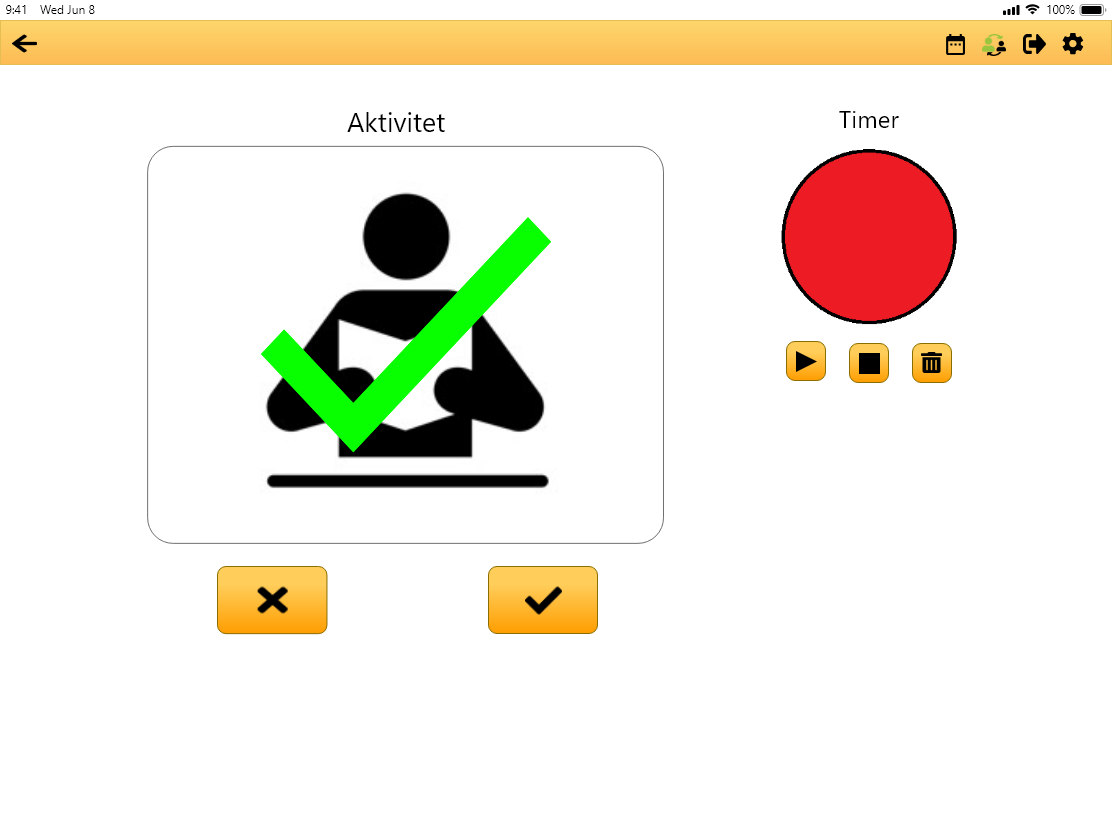
\includegraphics[width=1\linewidth, height=5cm]{aktivitet_new_timer.png}
    \caption{New timer for activity}
    \label{fig:activity_new_timer}
    \end{subfigure}
    \begin{subfigure}{0.5\textwidth}
        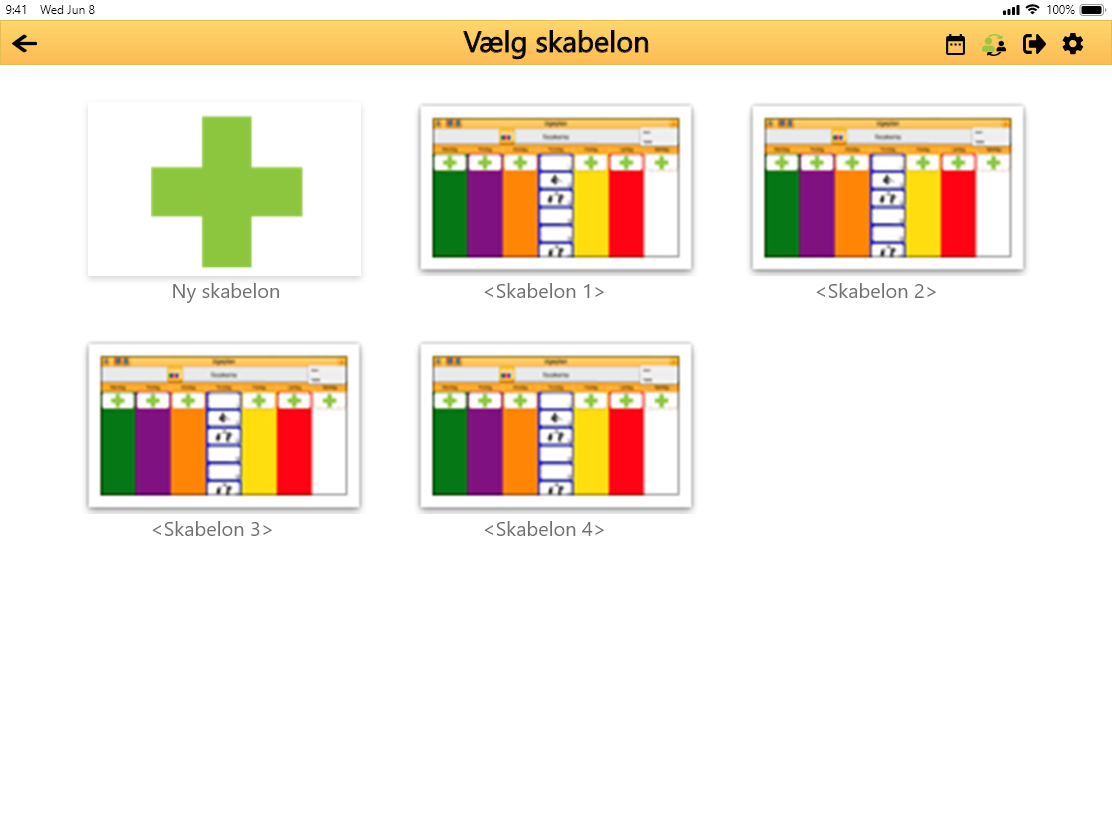
\includegraphics[width=1\linewidth, height=5cm]{ugeplan_skabelon.png}
    \caption{Week plan template select screen}
    \label{fig:weekplan_template_screen}
    \end{subfigure}
    \caption{New timer and week plan template selection prototypes.} 
    \label{activity_new_timer_and_weekplan_template_screen}
\end{figure}

\subsection{Copy week plan}
We refactored the prototypes for copying a week plan to other citizens to include the new dialog boxes to make the design consistent. In \autoref{fig:copy_weekplan} we see a confirmation dialog for copying a week plan. In \autoref{fig:copy_weekplan_confirm_copy} we see the screen for choosing which citizens the week plan should be copied to. 
\begin{figure}[H]
    \begin{subfigure}{0.5\textwidth}
    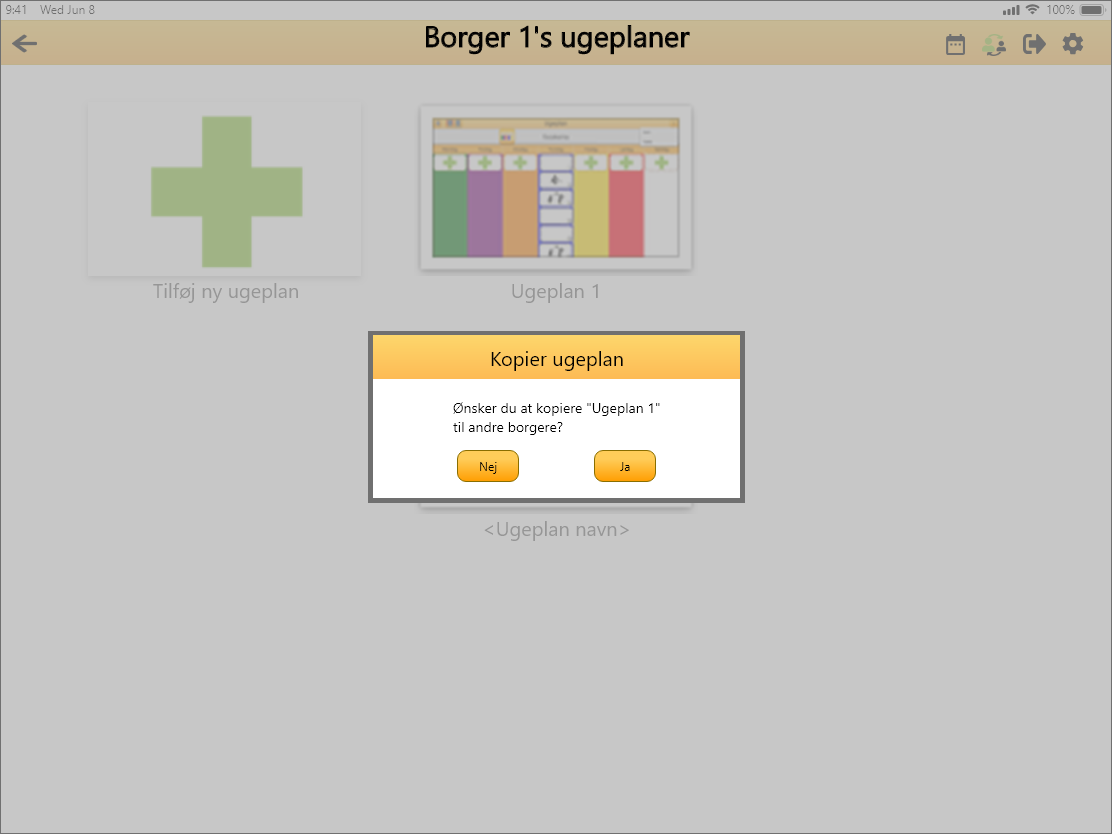
\includegraphics[width=1\linewidth, height=5cm]{copy_weekplan.png} 
    \caption{Copy week plan dialog}
    \label{fig:copy_weekplan}
    \end{subfigure}
    \begin{subfigure}{0.5\textwidth}
        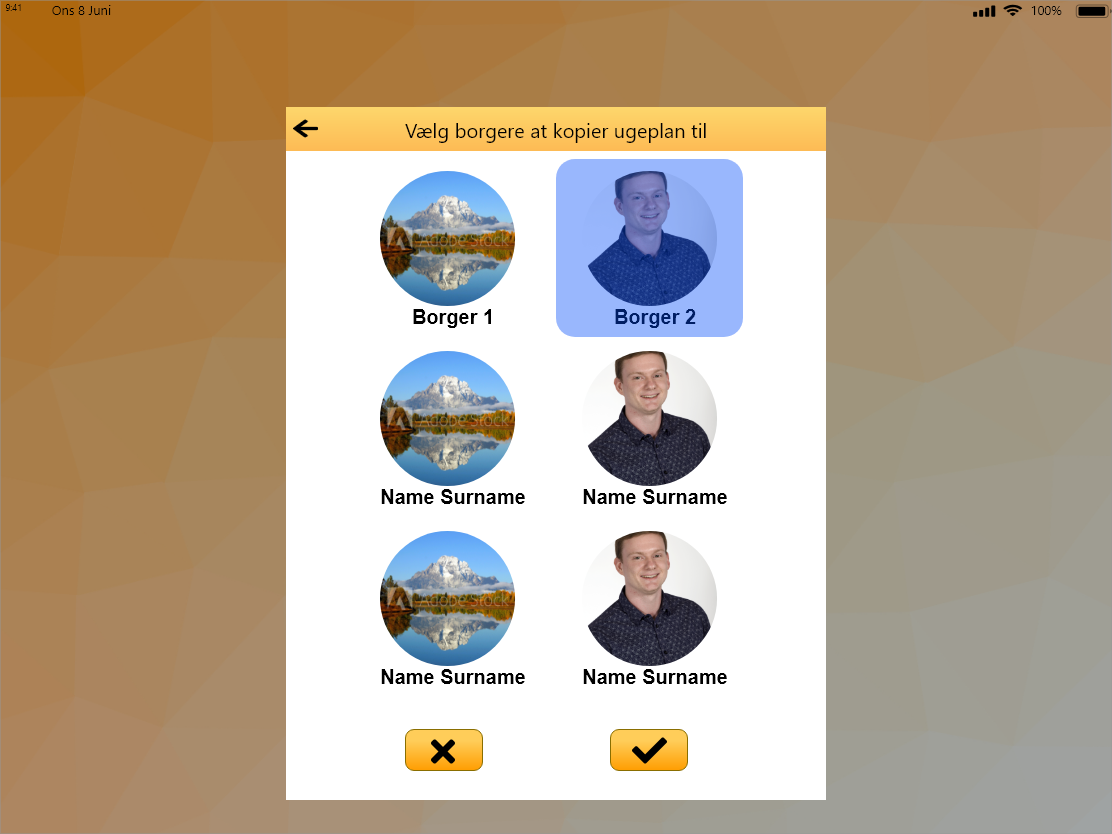
\includegraphics[width=1\linewidth, height=5cm]{copy_weekplan_confirm_copy.png}
    \caption{Choose citizens to copy week plan to}
    \label{fig:copy_weekplan_confirm_copy}
    \end{subfigure} 
    \caption{The dialog and citizen selection for copying a week plan.}
    \label{fig:copy_weekplan_confirm_copy_and_copy_weekplan}
\end{figure}
\noindent
Finally, in \autoref{fig:copy_weekplan_confirmed} we see the confirmation dialog when the week plan is successfully copied.

\begin{figure}[H]
    \centering
    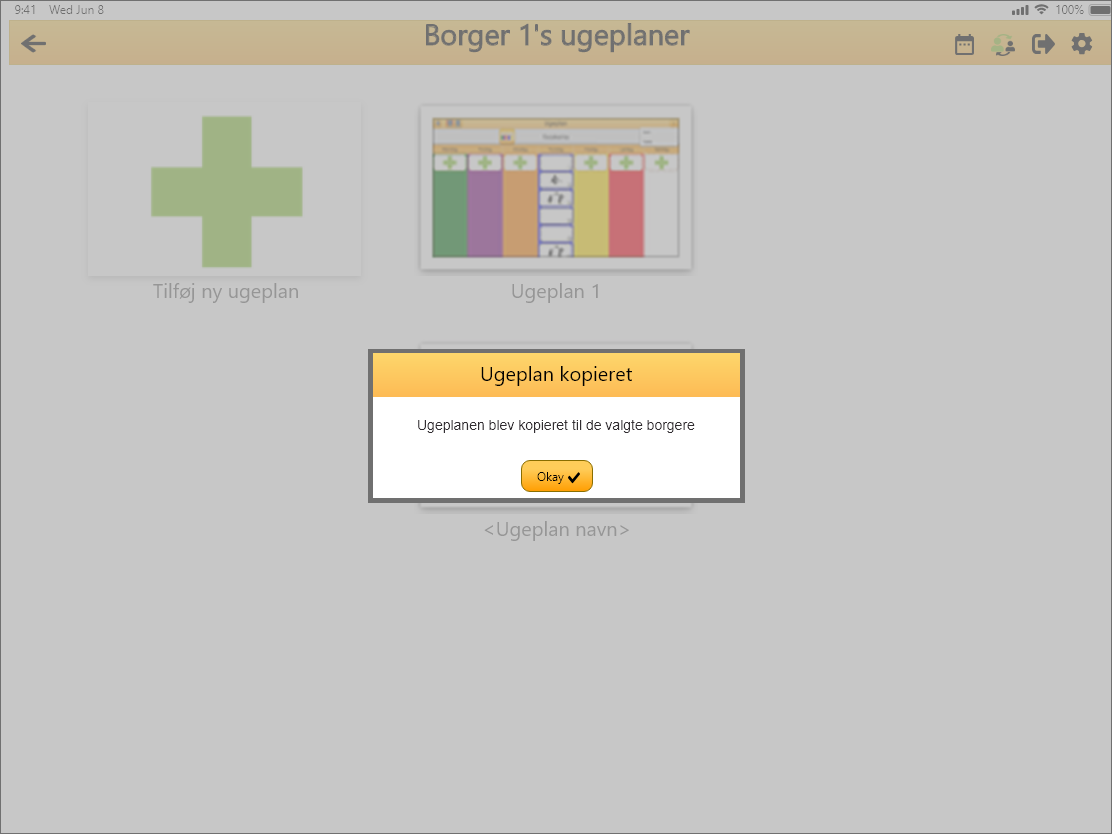
\includegraphics[width=0.5\linewidth]{copy_weekplan_confirmed.png} 
    \caption{Week plan copied confirmation screen}
    \label{fig:copy_weekplan_confirmed}
\end{figure}

\subsection{Copying of activities}
Here we created two different versions of prototypes that show how activities are copied between weekdays.
This is because we were unsure of what the customer would like, so we created different versions to show them.
The dialog with the checkboxes has the advantage of being able to copy to more than one day at a time.
\begin{figure}[H]
    \begin{subfigure}{0.5\textwidth}
    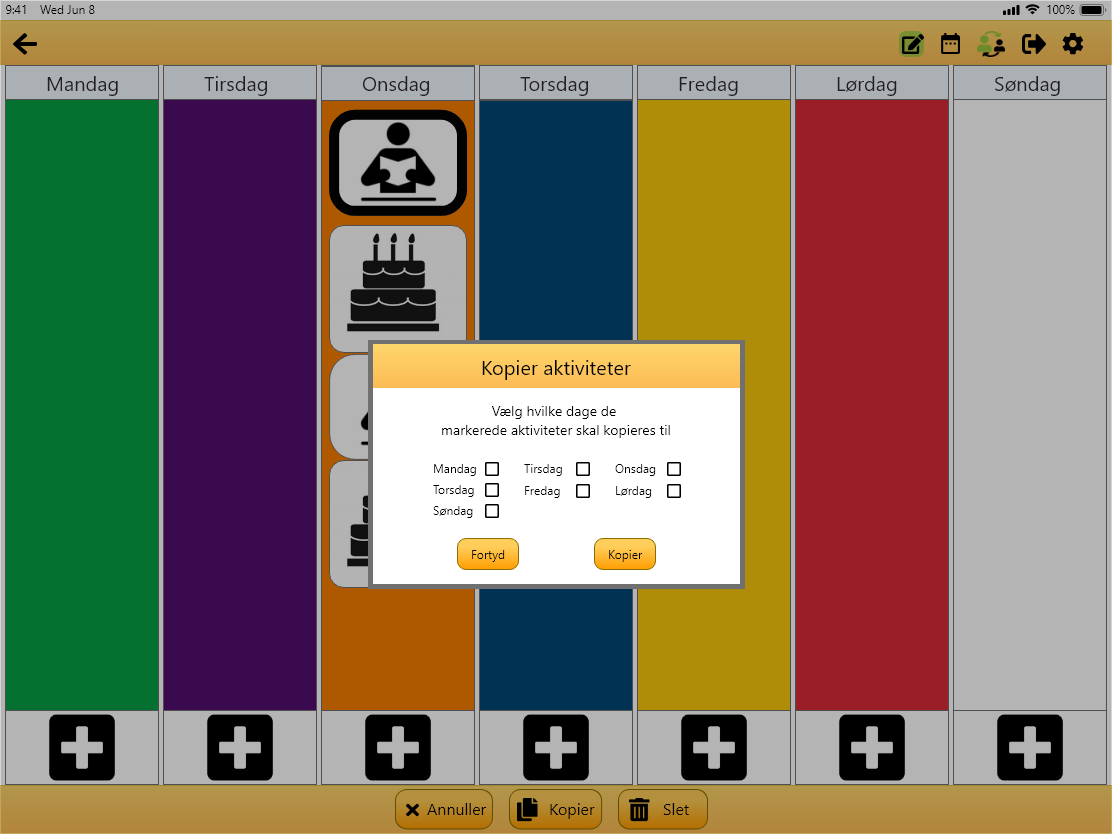
\includegraphics[width=1\linewidth, height=5cm]{mark_mode_copy_checkbox.png} 
    \caption{Copy activities dialog with checkboxes}
    \label{fig:mark_mode_copy_checkbox}
    \end{subfigure}
    \begin{subfigure}{0.5\textwidth}
        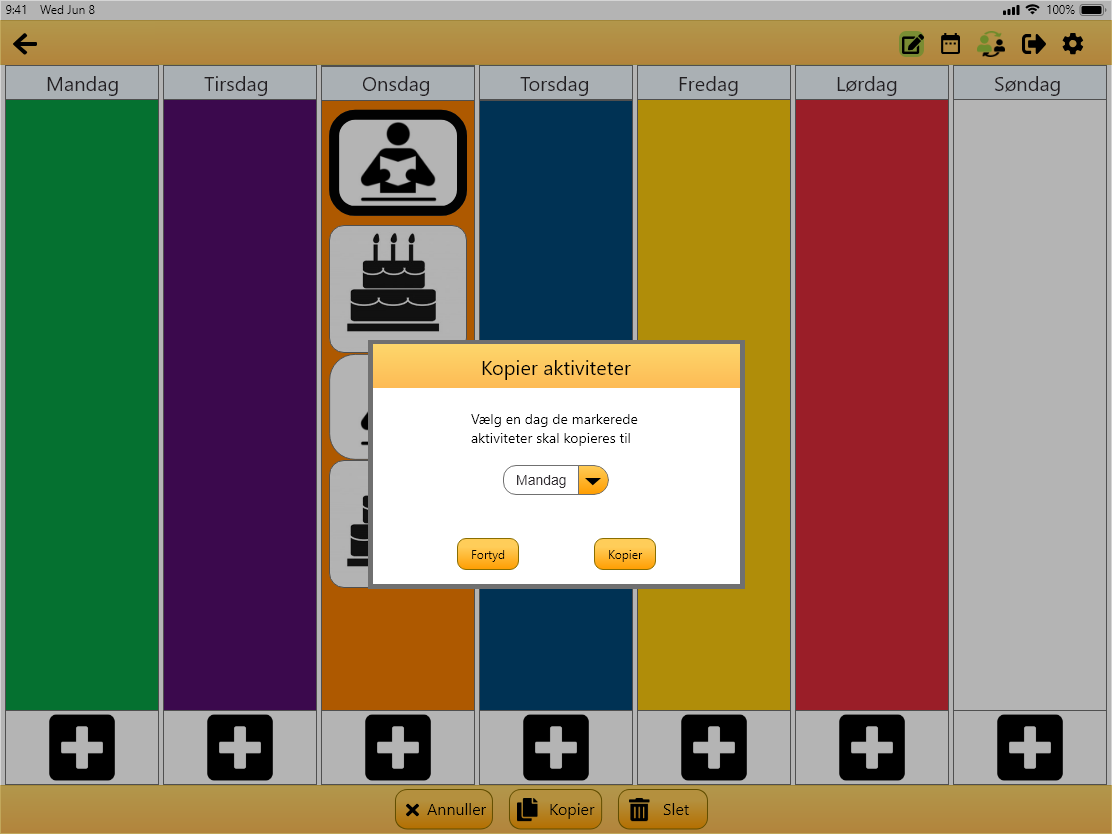
\includegraphics[width=1\linewidth, height=5cm]{mark_mode_copy_dropdown.png}
    \caption{Copy activities dialog with dropdown}
    \label{fig:mark_mode_copy_dropdown}
    \end{subfigure} 
    \caption{The two options for copying activities.}
    \label{fig:mark_mode_copy_dropdown_and_checkbox}
\end{figure}



\subsection{Adding new pictograms}
The customer wanted the option to add their own pictograms if they could not find the one they needed.
They suggested being able to add from the gallery of the phone or tablet, or by taking a picture directly.
We created a few prototypes this sprint that show how this could work.
First, in \autoref{fig:pictogram_bottom_bar}, we needed to create a way to go from the pictogram search to a screen where the user could choose pictures from their gallery.
A bottom bar with two buttons was enough for this.
In \autoref{fig:pictogram_add_gallery} we see the prototype for the screen where you can add photos from the gallery, and enter a name for the pictogram.
\begin{figure}[H]
    \begin{subfigure}{0.5\textwidth}
    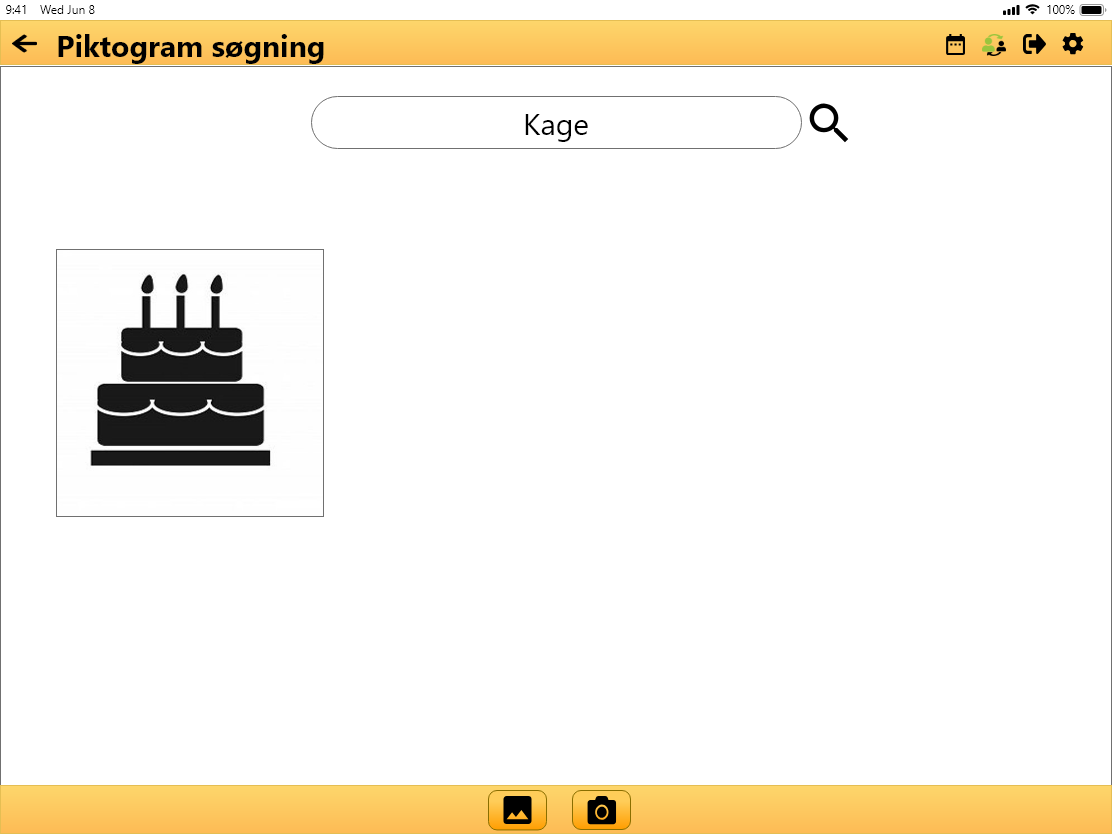
\includegraphics[width=1\linewidth, height=5cm]{pictogram_bottom_bar.png} 
    \caption{Pictogram search with bottom bar}
    \label{fig:pictogram_bottom_bar}
    \end{subfigure}
    \begin{subfigure}{0.5\textwidth}
        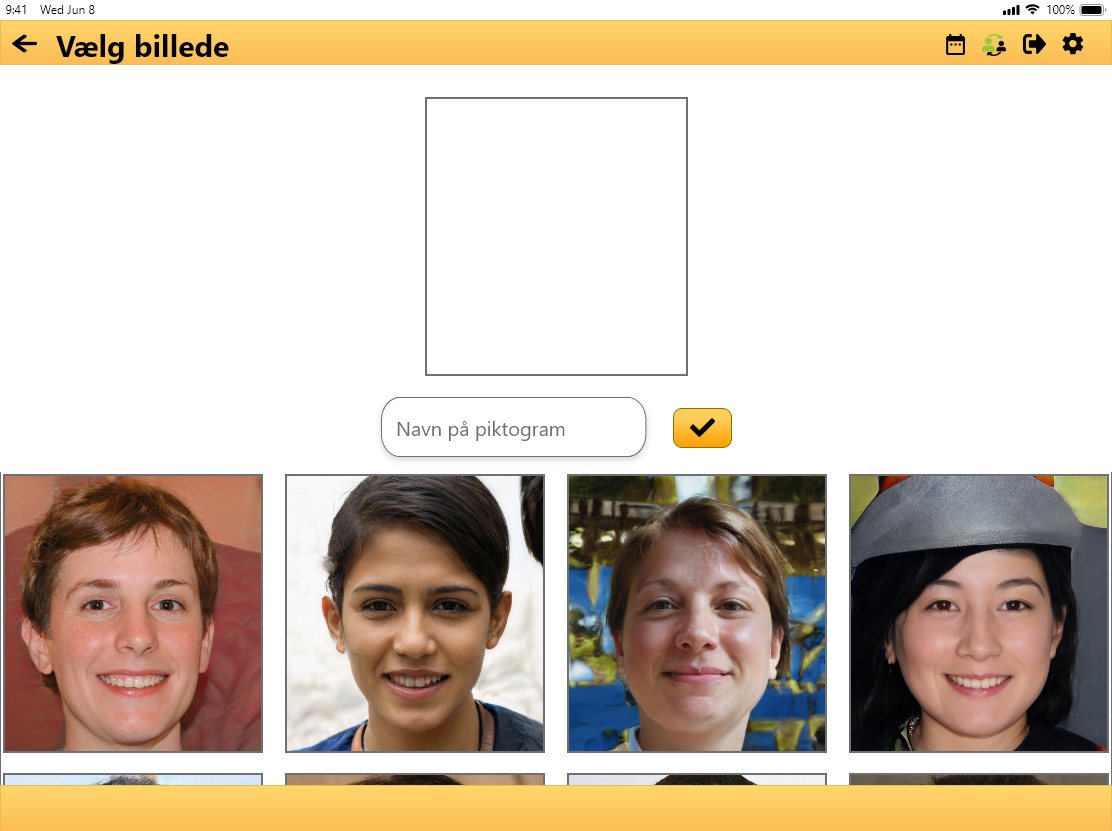
\includegraphics[width=1\linewidth, height=5cm]{pictogram_add_gallery.png}
    \caption{Screen for adding pictograms from gallery}
    \label{fig:pictogram_add_gallery}
    \end{subfigure} 
    \caption{Choosing to add a new pictogram, and the way we envision the screen should look.}
    \label{fig:pictogram_bottom_bar_and_pictogram_add_gallery}
\end{figure}
\noindent
In \autoref{fig:pictogram_add_camera} we see the screen where the user can add a pictogram from the camera, give it a name and then add it by clicking the checkmark to save it to the week plan.

\begin{figure}
    \centering
    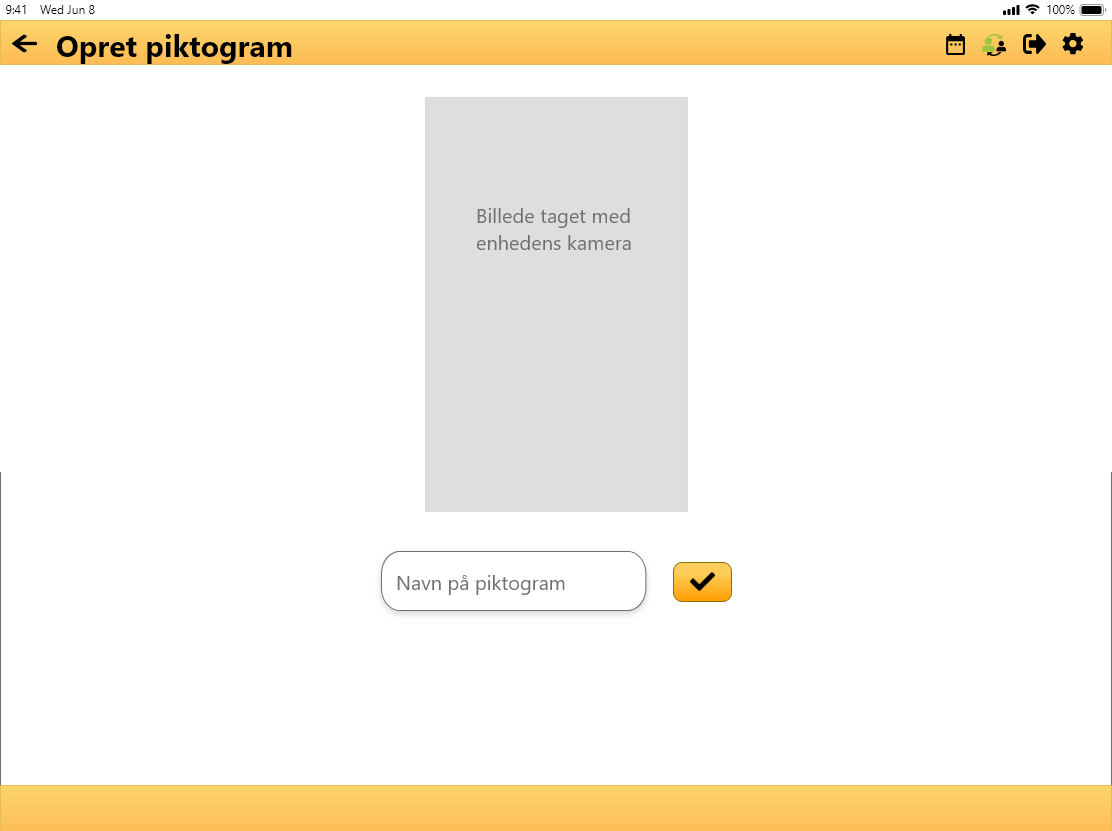
\includegraphics[width=0.5\linewidth]{pictogram_add_camera.png}
    \caption{Screen for adding pictogram by taking a picture with the device}
    \label{fig:pictogram_add_camera}
\end{figure}
\section{Release 2019S3R1}
For the release in this sprint all groups of GIRAF had a release preparation period for the last two days of the sprint. 
When the release preparation started, we expected every user story in the sprint to be finished and merged into develop. 
The ones that were not ready did not get included in the release. The release branch was then created from the develop branch.
The user stories that did not make it in time for the release can be seen in \autoref{table:unfinished-user-stories-sprint-3}.

\begin{table}[H]
    \small
    \begin{tabular}{|p{3.5cm}|p{9cm}|}
    \hline
    Issue ID        & User story   \\ \hline
    Weekplanner \#57  & As a guardian I would like to be able to remove an activity from the week plan so that cancelled activities can be removed from the citizens plan \\ \hline
    Weekplanner \#155 & As a guardian I would like to see the icons of a citizen on the choose citizen screen so that I can quickly identify them \\ \hline
    Weekplanner \#157 & As a user I want to be prompted an error message when failing to login correctly during a change from guardian to citizen \\ \hline
    \end{tabular}
    \caption{User stories that did not finish in time for the release}\label{table:unfinished-user-stories-sprint-3}
\end{table}

For the preparation, all groups of GIRAF sat together and systematically went through each new feature to see if they worked as expected. We did this as a result of \autoref{sec:sprint-2-retrospective} to make communication a lot smoother during release preparation.
The way it was done was by having each group review a couple of user stories that they had not developed themselves and check for bugs or inconsistent design. 
We created a checklist that the groups could used when testing the features.
\begin{itemize}
    \item Can the screen be reached through navigation in the application?
    \item Can you perform all the functionality defined in the issue?
    \item Can it be used without crashing?
    \item Does it run without bugs?
    \item Does it still look acceptable if you change to a new device or change orientation?
\end{itemize}
Bugs were reported on Github by the groups, and we, as the PO group, assigned other groups to solve these bugs.
All groups of GIRAF then sat together and solved the bugs by branching out from the release branch and merging into it again when they had solved the bug. 
We still had two code reviewers and a PO reviewer for each pull request during release. 
If the groups had any questions regarding design or functionality, we as PO group were always available to answer questions which was one of the benefits of having a release preparation together.
\\\\
When all the most critical bugs had been fixed, we held a release party where each group had a chance to present the functionality that they had been working on during the sprint. 

\section{Sprint review}
The sprint review meeting was cancelled during this sprint. 
This was due to it being too similar to the stand up meetings, and therefore it seemed unnecessary. 
We still evaluated how many of the user stories were completed and which were incomplete.
Most user stories were completed within the sprint with 5 user stories being incomplete.    
The user stories for sprint 3 and their status can be seen on \autoref{table:sprint-3-review}.
\begin{longtable}{|p{2.9cm}|p{7cm}|p{2cm}|p{2cm}|}
    \hline
    Issue ID        & Tasks                                                                                                                                                                                    & Assigned to  & Status   \\ \hline
    Weekplanner\#45 & As a citizen I would like to view details about the currently ongoing activity (such as time left and only the associated pictogram) so that I know what is happening and how long is left & Group 13   & Completed         \\ \hline
    Weekplanner\#53 & As a guardian I would like to be able to re-order the activities in a week plan, so that I can easily re-prioritize the activities for the citizen                                      & Group 9       & Completed         \\ \hline
    Weekplanner\#57 & As a guardian I would like to be able to remove an activity from the week plan so that cancelled activities can be removed from the citizens plan                                    & Group 13         & Completed         \\ \hline
    Weekplanner\#92 & As a developer I would like the application to use a default font so that I can easily change it                                                                                       & Group 10       & Completed     \\ \hline
    Weekplanner\#106 & As a user I would like to get a response when my search request times out so that I know what is going on                                                                             & Group 2        & Completed    \\ \hline
    Weekplanner\#112 & Entering an incorrect password when changing from citizen to guardian logs out the user                                                                                                  & Group 2     & Incomplete    \\ \hline
    Weekplanner\#125 & Exception thrown when rendering WeekPlanScreen, issue \#44                                                                                                                             & Group 10      & Completed   \\ \hline
    Weekplanner\#132 & As a user I would like to be able to switch between guardian and citizen mode so that I can only access the parts of the system that I should be able to                            & Group 2          & Completed    \\ \hline
    Weekplanner\#133 & As a guardian I would like to be able to logout when I am on the choose citizen page so that I can return to the login page                                                              & Group 10    & Completed    \\ \hline
    Weekplanner\#137 & A loading spinner should be shown when logging in (waiting for response from API).                                                                                                    & Group 9        & Completed     \\ \hline
    Weekplanner\#138 & Show an alert when trying to log in with the wrong information                                                                                                                         & Group 9       & Completed    \\ \hline
    Weekplanner\#146 & Change buttons on activity screen                                                                                                                                                    & Group 8         & Incomplete    \\ \hline
    Weekplanner\#149 & Change button on Notify Dialog                                                                                                                                                        & Group 8        & Completed    \\ \hline
    Weekplanner\#157 & As a user I want to be prompted an error message when failing to login correctly during a change from guardian to citizen                                                             & Group 2        & Incomplete    \\ \hline
    Weekplanner\#158 & As a developer I would like a default widget for confirmation dialogs.                                                                                                                  & Group 9      & Completed    \\ \hline
    Weekplanner\#165 & Change buttons on ConfirmDialog                                                                                                                                                        & Group 8       & Completed    \\ \hline
    Weekplanner\#166 & Logout button needs to use Confirm Dialog                                                                                                                                             & Group 9        & Completed     \\ \hline
    Weekplanner\#181 & The timer on the activity screen does not work                                                                                                                                         & Group 8       & Completed    \\ \hline
    Wiki\#34         & Migrate the WEB-API to Docker and document the work                                                                                                                                     & Group 12     & Incomplete    \\ \hline
    Wiki\#35         & Migrate the MySQL Database to Docker and document the work.                                                                                                                            & Group 12      & Complete   \\ \hline
    Web-API\#6      & Considering updating frameworks in web-API                                                                                                                                            & Group 12        & Complete    \\ \hline
    Web-API\#9      & Make new endpoint to get all week plans for a citizen in a single request so that we do not have to make a new request for each week plan                                                & Group 11        & Incomplete    \\ \hline
    \caption{Status of all user stories for sprint 3.}\label{table:sprint-3-review}
\end{longtable}


\subsubsection{Review of internal goals}
All the sprint goals for sprint 3 were completed.
The implementation of the different user stories were previously described in \autoref{sec:sprint-3-our-stories}.
\begin{table}[H]
    \centering
    \begin{tabular}{|l|l|}
    \hline
    Goals:                            & Status        \\ \hline
    Implement Weekplanner\#92         & Completed      \\ \hline
    Implement Weekplanner\#125        & Completed      \\ \hline
    Implement Weekplanner\#133        & Completed      \\ \hline
    Conduct a usability test          & Completed       \\ \hline
    Prepare a release                 & Completed         \\ \hline
    Prepare introduction for sprint 4 & Completed                        \\ \hline
    \end{tabular}
    \caption{Our internal goals in sprint 3 and their status.}
    \label{PO-goal-sprint-3-status}
\end{table}

\section{Sprint retrospective}
\chapter{Sprint 4}
\section{Sprint goals}
\section{Sprint review}
For this sprint, as mentioned in the introduction in \autoref{sec:sprint-4-introduction}, we delegated the user stories to the different groups to make sure that the most necessary stories would be completed. There were also some leftover user stories from sprint 3 that the development groups had to finish.
\\
The user stories for sprint 4 and their status can be seen on \autoref{table:sprint-4-review}.
\begin{longtable}{|p{2.9cm}|p{8cm}|p{2cm}|p{2cm}|}
    \hline
    Issue ID        & Tasks                                                                                                                                                                                    & Assigned to  & Status   \\ \hline
    Weekplanner\#2 & As a citizen I want a time timer so that I know how long is left of my current activity                                                                                                   & Group 9      & Completed  \\ \hline
    Weekplanner\#58 & As a guardian I would like to be able to mark an activity as cancelled so that I can let the citizen know that an activity has been cancelled                                            & Group 8      & Completed   \\ \hline
    Weekplanner\#59 & As a guardian I would like to be able to cancel and copy multiple activities at once by marking them so that I don't have to manually do it for each activity I want to change           & Group 13     & Completed   \\ \hline
    Weekplanner\#61 & As a guardian I would like to be able to add a timer to an activity so that the citizen can see how much time is to be spent on this activity                                            & Group 9      & Completed    \\ \hline
    Weekplanner\#62 & As a guardian I would like to be able to remove a timer from an activity so that the activity is no longer time specific                                                                 & Group 9      & Completed    \\ \hline
    Weekplanner\#112 & Entering an incorrect password when changing from citizen to guardian logs out the user                                                                                                 & Group 2      & Completed    \\ \hline
    Weekplanner\#128 & When changing from citizen to guardian, the password is saved in the input field                                                                                                        & Group 11     & Completed    \\ \hline
    Weekplanner\#135 & As a guardian, I would like a way to add pictograms by choosing an image from my phone gallery so that I can quickly improvise if the system does not have the activity I want          & Group 11     & Completed   \\ \hline
    Weekplanner\#157 & As a user I want to be prompted an error message when failing to login correctly during a change from guardian to citizen                                                               & Group 2      & Completed    \\ \hline
    Weekplanner\#198 & As a guardian I would like to be able to delete week plans so that I can avoid clutter and not be overwhelmed                                                                           & Group 13     & Completed    \\ \hline
    Weekplanner\#214 & Change buttons on NewWeekplanScreen                                                                                                                                                     & Group 8      & Completed    \\ \hline
    Web-API\#9 & Make new endpoint to get all weekplans for a citizen in a single request so that we dont have to make a new request for each weekplan                                                                                                                                                      & Group 11      & Completed    \\ \hline
    Web-API\#17 & New Add and Delete Activity Endpoints                                                                                                                                                      & Backend metagroup     & Completed    \\ \hline
    Web-API\#18 & An update activity endpoint                                                                                                                                                      & Group 13     & Completed    \\ \hline
    Web-API\#29 & Unable to log in on the admin panel                                                                                                                                                       & Group 12     & Completed    \\ \hline
    Web-API\#32 & Updating timer through the update activity endpoint and adding Timer to the database                                                                                                                                                       & Group 9     & Completed    \\ \hline
    \caption{Status of all user stories for sprint 4.}\label{table:sprint-4-review}
\end{longtable}
\noindent
As can be seen on \autoref{table:sprint-4-review}, all of the user stories were completed. Furthermore, it should be mentioned that for each \texttt{web-API} issue completed that introduced a new endpoint, there was also an equivalent endpoint made in the \texttt{API-client} to allow communication between the back end and front end.

\subsection{Review of our internal goals}
All the sprint goals for sprint 4 were completed.
\begin{table}[H]
    \centering
    \begin{tabular}{|l|l|}
    \hline
    Goals:  & Status \\ \hline
     Create prototypes for new user stories for next year & Completed\\ \hline
     Write advice for next year's PO  & Completed  \\ \hline
     Conduct usability test & Completed  \\ \hline
     General documentation for handover & Completed \\ \hline
     Prepare final release & Completed  \\ \hline
    \end{tabular}
    \caption{Goals for the PO group in sprint 4}
\end{table}


\section{Sprint retrospective}
\include{sections/conclusion/conclusion}
\chapter{Appendix}
% PO:
Okay så, vi har ligesom fået delt spørgsmålene ind i sådan tre kategorier. 
De første de bliver sådan lidt med for at forstå hvordan i lige nu benytter IT i hverdagen, og så kommer der sådan noget specifikt til GIRAF projektet, og så har vi lige nogle sådan rent proces relaterede - vores gruppe og jer som kunde imellem.
Det første vi har tænkt på, det er, sådan i store træk, hvordan benytter i IT i hverdagen lige nu?   

Emil: 
Ja, og det er jo, der skal vi lige sådan snævre det lidt ind. 
Jeg fortalte jo også hvor bredt vi egentligt benytter IT på skolen, ikke også, indenfor alle områder. 
Det gennemsyrer jo en arbejdsplads som en specialskole, men er det med særlig fokus på det her omkring struktur og kommunikation, eller?

PO: 
Ja, lige præcis.
Som støttemiddel til eleverne.

Emil:
Ja.
Hvordan bruger vi det der?
Jamen vi bruger det ikke sådan, hvad kan man sige, ensrettet.
Det er meget fra klasse til klasse, med det personale der tilfældigvis er i klasserne hvad de har med sig af erfaring og hvad det er de har for nogle konkrete elever og hvad det ligesom kan løse af udfordringer i hverdagen.
Det er med det perspektiv hvor det er.
Så det er på den måde er det meget forskelligartet hvordan det bliver brugt.
Vi har nogle klasser hvor at de kører for eksempel, dagstruktur bliver kørt sådan fælles på en tavle, så alle elever får det samme, ikke også, som sådan et fælles opmærksomhedspunkt.
Og andre har hver deres system hvor måske nogle af dem har det sådan elektronisk. 
Så, ja.

PO:
Lige for at følge op til det der - er det sådan at hver klasse, er det kun delt ind i sådan årgang og sådan nogle ting der eller er det også hvordan de er som personer?

Emil:
Det er et godt spørgsmål.
Selvfølgelig så har, så går dem der går til afgangsprøve jo ikke med nogle som ikke har talesprog, det er jo ikke sjov undervisning.
Så, vi har på skolen delt dem op i tre afdelinger.
En afdeling som der faktisk ikke engang ligger i Hammer Bakker, men som ligger ude i Sulsted der hedder Agernhuset for vores højt begavede, normal begavede unge som der følger almindelige skolematerialer.
De går ude i den afdeling, og så har vi sådan en hovedafdeling hvor der er en mellemgruppe, både for dem der er så, ja, dem der ikke lige passer direkte i nogen af dem, og så er der dem der næsten ingen talesprog har.
Mellemgruppen den er rimelig bred. 
Der er nogle som hvor deres sprog det er sådan rimeligt upåfaldende, men de har måske nogle massive autismevanskeligheder omkring det sociale, for eksempel, og ja.
Der kan være mange ting i det, men så hver afdeling har så tre trin.
En udskolingsgruppe, og en indskolingsgruppe og et mellemtrin. 
Så man finder ud af sådan hvor passer de henne sådan kognitivt og hvad for nogle skolematerialer kan de følge, ikke også, og så placerer man dem i afdelinger efter det, og så placerer man dem i klasse efter alder.
Det skal være en af de tre trin. 
Så der er rimelig stor spredning i vores, det er klart når der er nogle der går i både børnehaveklasse med nogle der også går i trejde.
Så, ja, men sådan er det.
Det er jo små grupper til gengæld, så vi differentierer jo hæftigt i hvad de får af undervisning.

PO:
Ja okay.
Har de sådan, alle eleverne, har de iPad eller tablet til rådighed?

Emil:
Ja.
Alle elever har iPads til rådighed. 
Det er helt fast, og nogle har endda mere end en iPad til rådighed.

PO:
Er det noget de sådan er rimelig kompetente i at bruge?

Emil: 
Alle er 100\% kompetente i iPads, ja.
Jeg tror faktisk der er en enkelt klasse der så ikke har iPads ude ved Agernhuset, men de har fået PCer fordi de skal bruge det i forhold til deres afgangsprøve, og man kan kun få en enhed.
Generelt så er det iPads der, for 85\% af alle vores elever. 
Og dem kan alle finde ud af at bruge, selv de aller dårligste kan finde ud af at trykke på en iPad.
Ja.
Det er noget af et frmeskridt i forhold til da det var på PC med mus, den der hvor du skal styre noget og klikke op på en skærm.
Der var det ikke alle der kunne bruge computer, men alle kan bruge en iPad.

PO: 
Er det sådan nogle specille områder du sådan i hverdagen har tænkt at, det kunne være smart hvis det her det var digtaliseret?

Emil:
Ja. 
Godt spørgsmål.
Altså, vi er jo sådan en arbejdsplads og et område med rigtig mange traditioner også, hvor at ,am jo gør meget man plejer og har erfaring for at fungere. 
Så det, man kan jo sige at specialområdet er jo generelt, selvom de også er med på at udvikle mange tinge, så er de også meget traditionsbundne. 
Så det kan gøre det lidt svært at rykke.
Altså, jeg synes egentligt, altså det er nogle af de områder jeg har været inde på omkring kommunikation og struktur hvor jeg tænker at der er, det er mest meningsfult at bruge det i nogle særlige situationer.
Vil jeg sige.
Det er, der kan man sige, de programmer der kan altid gøres bedre end det de er. 
Der er ulemper ved dem alle sammen. 
De har hver deres fordele og hver deres ulemper.
så vi er hele tiden sådan på afsøgning af, hvad er det, hvor er det vi får mest for pengene.
Hvad, ja, hvad rammer dem bedst.
Og det skifter også hele tiden.
Det gør det.
Jeg tror egentligt umiddelbart at vores største udfordring, det er personalet som brugere, umiddelbart.
Så jo mere nemt det er at gå til for personalet, jo større vil impact kan du få på det.

PO:
Må jeg lige høre, nu når du siger det der, er det sådan at lærer personalet op i hvordan man bruger de der apps der?

Emil:
Ja.
Det er forskelligt også, nogle, der er jo nogle de kan jo gå til det med det samme ikke? 
Og så har vi også nogle der har rigtigt svært ved det.
Det er bare hvis du skal bruge noget, hvis du skal støtte en elev på noget der er så vigtigt som at de trives i deres hverdag og kan have en forudsiglighed og struktur, ikke også, så er det jo vigtigt at alle voksne omkring barnet kan finde ud af at tilgå det her og støtte barnet med det.
Det nytter ikke noget det kun er halvdelen.
Så er det bedre at bruge noget andet.
Så derfor, så kan man sige, er det meget brugervenligt så er der stor sandsynlighed for at alle vil kunne gå ind og gøre det.

PO:
Er det noget, sådan de apps som i har nu for eksempel, de gør noget for at få, eller sådan gør det nemmere for jer?
Der er Selvfølgelig brugervenlighed i appsne, men er det også sådan guides inde i appsne eller sådan noget?

Emil: 
Faktisk så vil jeg sige, at den der som vi nu lige forsøger at tilkøbe, det irriterer mig enormt meget at jeg ikke kan huske det.
Hvad er det den hedder?
Det er ikke Showmyday.
Nå, den vandt faktisk, vi havde, vi har haft en større afsøgning siden efteråret hvor vi så, hvad er der egentligt overhovedet af muligheder?
Og så skriver vi det ind.
Vi havde to tilbage til sidst. 
Dene ene den var billig, og den anden var sådan en mellemklasse app.
Vi valgte den vi valgte primært fordi at der er så ekstremt mange guides på YouTube til hvordan man skal bruge det.
Så det er mega nemt for personalet at gå ind, den er simpelthen, når du åbner den så er den utrolig intuitiv og nem at gå til for de fleste, og har man brug for støtte er støtten rigtig nem at få.
Det vil også være i forhold til forældre og sådan noget, ikke også, at de kan, man kan henvise til har du set der er YouTube klip nummer 35, der kan du se lige præcis det der du spørger om.
Så det gør det nemt at få det, få hele barnets familie med omkring det, så det ikke er en person i teamet der skal vejlede både kollegaer og forældre og altså det bliver en kæmpe arbejdsbelastning.
Så det var faktisk det den vandt på. 
Den anden den tabte især på at den kun kørte på Android. 
Det er også lidt en ulempe. 
Eller også så kørte den kun på Apple, og så var der nogle af vores elever der havde... 
Nej den kørte faktisk kun på iOS, og så var det sådan at vi har nogle elever der ville have rigtig stor gavn af den som har Android telefoner og ikke ville kunne bruge den der.
Hvor den anden vi købte den kører på begge systemer.
Så det er et stort plus at der er den fleksibilitet. 

PO:
Så det er en stor bonus hvis der var noget dokumentation, for eksempel i videoformat, tilgængeligt for GIRAF?

Emil:
Ja, klart.
Noget guide.
Altså man skal tænke at det skal være nemt at gå til og der skal være, du skal kunne hente støtte nogen steder, ja.

PO:
Er det sådan hovedsagligt kun for guardians, eller er det også sådan for citizens? At de skal have det der i videoformat, eller er det simpelthen personalet man helst bare skal?

Emil:
Det kan jo være, det kommer jo an på hvordan man laver det.
Så det behøver det jo ikke være.
Det kan også bare være hjælpefunktioner der er gode og så noget derinde, så det synes jeg er svært at svære entydigt på.
Hjælpen skal bare tænkes ind.
Man skal tænke ind at lærere og pædagoger er ikke nødvendigvis gode til IT.
Overhovedet.
Det er bedre at tænke det modsatte. 
Og så er der nogle der har rigtigt nemt ved det, men sådan er det.
Det skal designes til ens mormor.
Så noget jeg egentligt også synes vi mangler lidt, det er apps der kan, jeg viste det der med timeren i så med uret, det er jo sådan en app, det er jo en købe-app, jeg tror den koster en halvtredser eller sådan noget, og den er god fordi den ligner rigtig meget det ur vi har.
Nogle forskellige repræsentationsformer af tiden der går, det er faktisklidt en mangelvare synes jeg.    
Jeg synes egentligtpgså det er halvdyrt for et program der er meget, meget simpelt at lave. 
Det der det kan satan edme ikke tage ret meget tid at lave det kode til og køre den der ned.
Det synes jeg faktisk at vi har haft tænkt lidt ind i GIRAF, hvordan skulle tiden repræsenteres.
Det er der tænkt lidt for lidt over synes jeg.  
Det er faktisk et ret vigtigt issue for vores elever. 

PO:
Hvordan tænker du så man kunne repræsentere tid? 
Jeg tænker umiddelbartat det var noget der ville kunne være svært.

Emil:
Det kunne jo være alt fra, der er sådan lidt forskellige systemer man bruger, der er nogle der arbejder med sådan noget der hedder quarter-dots hvor det er sådan nogen røde prikker der ligesom forsvinder væk.
Du kender det jo også, det kunne også være sådan en bar som du har når et stykke software det loader som der går ned.    
Så det kan tænkes på mange måder, det er bare, det behøver ikke nødvendigvisvære den der røde cirkel.
 
PO:
Vi har også, jeg ved at der har været snak om lige nøjagtigt den feature med sidste års studerende, hvor de blandt andet har haft noget timeglasrepræsentation eller bare som digital tid.

Emil:
Ja, vi har også nogle der bruger almindelige timeglas, det er der også nogen der er glade for.
Det vil være rimeligtmeneingsfuldt at der var flere måder at gøre det på.
Det ser jeg i hvert fald ikke i ret mange software, at de har det. 

PO:
Er det så sådan for hvert barn at man skal kunne gp ind og vælge hvilken form de gerne vil se?

Emil:
Ja.
Det kunne også være at man havde dem, det er jo igen det der med hvor meget skal det være flettet sammen, og hvor meget skal det være selvstændige apps. 
Hvor man kan sige, for nogle børn ville det, hvis man bare havde en app der hed tidstageren eller hvad fanden man kunne kalde den, så havde du den gennem dagen på din iPad, hvor du kunne se nu skal du lige, nu skal du vænne dig, vi ved bare den her med batteriet den er super god til dig fordi du kender den fra din iPad.
Så den tæller ned eller hvad den gør, ikke?
Ja, eller quarter-dots eller en time timer så man ligesom har en lille pakke der med forskellige tidsrepræsentationer.  
Så kan det også være meningsfuldt selvfølgelig hvis du kan koble det sammen med aktiviteterne, at man kan se det i forbindelse med kalenderen. 
Ja, det er hvor integreret det skal være.   
Men tidsdelen, den synes jeg den mangler.

PO:
Der er et spørgsmål der relaterer sig til farver, hvor vi fik at vide at det var en international standard, er der sådan andre standarder man skal være opmærksom på, du lige kender til?

Emil: 
Nej.
Standarden er jo bare at det skal kunne tilpasses. 
Eller, farverne ja, det er en standard, det vil jeg sige, det nok er det. 
Så er der noget som er hyppigt brugt, som for eksempel ikonerne, hvor du tit bruger et system der hedder Boardmaker, som jo ikke er det eneste der findes på markedet, men som er rigtig, rigtigt udbredt indenfor autismeområdet.
Men altså, der kan tales godt og dårligt om dem, de bliver bare rigtigt meget brugt og der er også rigtigt mange elever der lærer dem at kende.
Det er jo så en anden ting, ikke, at de skal lære og forstå, hvad vil det sige, det der ikon som der viser en der for eksempel holder pause, at det ser sådan ud, og så skal jeg gøre sådan.
Hvor at det der med at forstå symboler det er jo lidt abstrakt og faktisk noget vores elever har svært ved, så der er meget udenadslære i det.
Så derfor er det ikke sådan noget man bare lige kan skifte rundt i mellem, men til gengæld tager du nogle af vores normalt begavede unge så synes de jo de er utroligt barnlige og grimme, og det er de jo også, det vil jeg give dem ret i.
Så jeg gjorde meget det i det tidligere projekt, der søgte jeg bare ikonerne på nettet og fandt nogle der var lidt mere pæne, cleane i deres, ja, den visualisering der var lavet. 
Det var mere spiseligt, vil jeg sige.
Det blev der taget godt imod. 
Så det er jo sådan den ene halv-standard man har, det er det Boardmaker der. 

PO:
I forhold til farver, hvordan, udover der er en standard, er det sådan noget de går op i, eller er det bare sådan at det skal ikke ændre sig?

Emil:
Nogle gør.
Nogle går op i det, nogle går ikke op i det.
Det andet, altså hvor kraftige de er i farven er nok mindre vigtigt.
Nu kan du se dem jeg lige har med der, ikke også, de er sådan meget farvefyldte eller farvemættede eller hvad man kan kalde det.
Men om de er mere nedtonede eller sådan, det tror jeg er mindre vigtigt.  
Så man kan godt arbejde med nuancerne tænker jeg, men farverne de er nu som de er.

16.00









\section{Summary of the project}\label{appendix:project-summary}
This is the sixth semester project for software engineering students at Aalborg University 2019.
It is a collaboration between seven software groups with 4-6 members.
This project is based around GIRAF, an application designed to help schools and kindergartens structure weeks for autistic children, and to help these children in their everyday.
The project collaborates with multiple institutions, ensuring customer contact is an essential part of the project.
An important aspect of the project is to get experience working with an existing codebase. 
The GIRAF project has been ongoing for multiple years, and as such, an understanding of previous years work has to be achieved.
The focus of GIRAF 2019 is to focus on the front end to make it more stable and aesthetically pleasing.
\\\\
For this semester the groups function as full stack groups.
This means each group has knowledge within all areas of the application.
To facilitate this, skills groups are established, consisting of a representative from each group.
These groups have an area of expertise, and it is the responsibility of the skill group member to convey the knowledge gained from the skill group to their official group.
There is also a dedicated process group, concerning itself with the processes used across the semester, and a dedicated product owner group, concerning itself with customer contact and ensuring the application is made to their specifications.
This report is made by the product owner group, and as such, focuses on customer contact as well as implementation.
\\\\
This semester is split into four sprints, for which we prepare a list of user stories and prioritize them based on customer contact.
Each sprint contains an initial planning meeting, where the user stories are presented and each group is assigned at least one user story.
Regular stand up meetings are held in each sprint to keep everyone up to date with the progress of the different groups.
When a sprint ends, a release candidate is created with the new functionality.
This release is then brought to a usability test with the customers, where they interact with the system to complete tasks we define.
The feedback we receive is then used to prepare the next sprint.
A sprint retrospective ends a sprint, and different aspects of the process are discussed to determine points of improvement.
\\\\
The project experienced difficulties initially, but proceeded smoothly after a change of framework to Flutter.
A new version of the GIRAF application was finalized after sprint 4 and uploaded to the \textit{Google Play Store}.
The product is a usable version of the weekplanner part of GIRAF, that allows a user to use pictograms to structure a day of activities.

\section{PO advice for next year's PO group} \label{appendix:PO-advice}
This document serves as a list of advice for the next PO group based on the experience we gathered throughout the semester.
The PO group's main responsibility is to communicate with the customers of the GIRAF project and document this interaction.
It is important that the customers' reactions, opinions and wishes for the application are documented, as these are the foundation for all the decisions that you, as the PO group, will take.
In the following sections we provide an in-depth description of how we advise customer contact to be handled, and how the information gathered should be used.

\subsection{Customer contact}
In the start of the semester Ulrik will most likely schedule some meetings with the customers which everyone should attend.
These serve to get the developers up to speed with what exactly the GIRAF project is and how the application is supposed to help people diagnosed with autism.
Before these meetings it is a good idea to contact the customers to try and arrange a time for a more secluded meeting where you, as the PO group, can ask more specific questions regarding functionality and design of the program.
The other groups should not be present for these meetings as it is your responsibility to relay this information to the other groups.
We arranged a meeting with Emil from Egebakken right after his initial presentation.
It is a good idea to get their phone numbers if possible, as it has been evident from our experience that communication through mail is often lacking and you might often not receive a response.
After this meeting you should have a good idea of what the customers want.
You can then start setting goals for what should be completed in the upcoming sprint, as well as for the whole semester.
\\\\
As soon as you have the start and end dates for you sprints solidified, you should contact as many customers as you can with dates for usability testing. 
We did this by sending a mail to every customer involved in the project.
Remember to schedule usability testing after your releases so that you have a working application for the customers to test and evaluate.
It is important that you ask the customers to confirm that they will participate in these tests.
If they do not respond you should try and contact them to see if they simply forgot to reply.
We did this by calling them on their phones or by calling their workplaces.
\\\\
It is very important to take notes and document all meetings with customers.
You will receive a lot of questions from the different developer groups about how functionality should be made and how it should look.
Therefore, it is always better to have written down exactly what the customers want so that you do not have to guess and then refactor later if you guessed wrong.
An issue we faced was that we thought it would be sufficient for a guardian to copy activities one day at a time, but when we showed prototypes to the guardians they were very adamant on having the functionality be able to copy to multiple days at once.
Another reason to document as much as possible is that the users' feedback is the foundation of all the user stories you are going to create.

\subsection{Creating user stories}
As the PO group it is your responsibility to create user stories.
User stories are created based on requests from the users.
We structured user stories in the following way:
\begin{itemize}
    \item As a ... I would like ..., so that ...
\end{itemize}
When creating a user story you should consider the amount of work that is needed for it to be completed, and whether or not it should be split into multiple smaller user stories.
We created user stories in the weekplanner repository on our GitHub page under the issue tab.
This made it easy to organize as user stories are uniquely numbered and can be put into milestones.
When creating a pull request it is easy to tag the user story so that it will be automatically closed when the pull request has been merged.
It also allowed us to assign them with tags such as "feature", and give them different priorities ranging from lowest to highest.
A user story should, if needed, contain a prototype that ideally has been approved by a customer and a further description of the problem.
We also had great success having one of the more experienced Flutter developers write a short technical comment explaining how they would structure the solution for the user story.
This gave the developers who were not as experienced with Flutter a better starting point.
\\
Below is an image of a user story.
\begin{figure}[H]
    \centering
    
\includegraphics[width=1.0\textwidth]{userStory.PNG}
    \caption{User story \#88 from sprint 2.}
    \label{fig:userstory}
\end{figure}
As you can see on \autoref{fig:userstory}, the user story has the number 88 and was created by the user Eduardsen.
It has the tags "priority: highest" and "type: feature" and is under the milestone called sprint 2.
In the right hand side you can see the profile picture of the developer currently assigned to implementing this user story.
\\\\
Another approach to creating user stories is when developer groups create feature requests.
In most cases these need to be rewritten into user stories if the problem they are describing has not been formulated correctly or adequately.
When creating user stories, take special care to ensure that your user stories are not written ambiguously and, if so, that you have the precise functionality that the users wanted explained within them.

\subsection{Prototypes}
One of the important tasks of the PO group is to create and maintain prototypes.
Prototypes should conform to the design guide which can be found on the Github Wiki-page.
PO groups from previous years had been using PowerPoint to create prototypes, but we found this process to be slow and require a lot of repetitive work.
Instead, we opted to use Adobe XD which reduced repetitive work and let us import the exact icons we used throughout the design guide, making the prototypes much more consistent.
During meetings with the customers you should show them the prototypes you have made since the last time you spoke.
It is a very good idea to get customer feedback so that you know you are headed in the right direction in relation to their expectations.
Prototypes are also helpful if developers have a creative way of interpreting a user story, as it allows you to show them how it should be with certainty.

\subsection{Distribution of user stories}
In the beginning of a new sprint you should present the goals of the sprint to all the other groups.
You should also present the user stories you believe correspond to these goals.
Afterwards, groups are free to take one or two user stories that they can start working on from the ones you presented.
These are the user stories that will help you reach the functionality defined in the sprint goal, and should be prioritized highly.
If a development group finishes their user stories before the sprint is over, they should be able to contact the PO group by writing or visiting the PO group to ask for a new user story to start implementing.
This should be done so the PO group can constantly keep track of the user stories currently being implemented.
We decided to continually update a board in our group room with the status of all development groups and their user stories which worked well.
\\\\
We chose to decide how to distribute user stories for the final sprint.
We did this because we had a lot of documentation tasks that needed to be done, and decided to distribute these as well to increase the likelihood of them being finished for next years groups.
Consider doing the same for final/short sprints to maximize value for the customer.
As you know which groups implemented which stories, and how productive the different groups are, you can use this to your advantage when distributing tasks.
User stories that relate to work done by a group previously should be delegated to that group.


\subsection{Communication with other groups}
During a sprint it is crucial to keep track of the status of other groups.
Certain user stories can be blocked by other user stories, and because of this you should regularly walk to the other group rooms and ask how their work is proceeding.
Being the PO group you should have a good overview of the developer groups' skills.
If a certain group is stuck with a user story you should ask other groups to help them complete it.
This is a great way to share knowledge and speed up development in some cases.
\\\\
Knowing what people are working on also gives you the advantage of knowing what files they are most likely making changes in.
This information can help you decide which user stories developer groups should take so that you reduce the amount of merge conflicts.


\subsection{Cooperation with process group}
A lot of the choices in regards to the process affects the work of the PO group.
Because of this it is essential that you communicate with the process group and ensure that you are in agreement about what is being planned.
For this semester we shared a group room with the dedicated process group, easily facilitating communication. 
You should attempt to do the same.

\subsection{Approval of designs}
We recommend enforcing that the PO group should be assigned to all pull requests that deal with the user interface of the application, as they are the group with the best understanding of how the customers interact with the system.
This means that the design should be consistent with the prototypes that have been approved by the customer, and be very intuitive for them to use.
It is a commonly known fact that software engineers are not designers and do not always think of user friendliness, so remember to keep them in check so the customers can actually figure out how to use the system.
This might be difficult for you too as it was for us, but try your best.
Some things we have noticed that you should pay special attention towards in design related PRs are: 
\begin{itemize}
    \item Good error messages should be shown to the user
    \item Icons are only used for \textit{one} thing
    \item The design should be consistent with the design guide
\end{itemize}

\subsection{Release preparation}
Be prepared that at the end of every sprint you will not have much time to finish your assigned user stories, because the last days of every sprint will be spent on preparing the release.
At the first release preparation we tried to get as many user stories included in the release as possible.
This meant that we were waiting for some groups to finish their user stories.
We realized that this was not feasible and that we had to make a concrete deadline.
This deadline had to be kept.
Even though one of the user stories just needed 10 minutes extra before it would be completed it would have to wait until next release to be included.
It was not feasible for us to keep delaying the release.
\\\\
When the deadline is reached, the release branch should be created.
We would cooperate with the process group to assign groups to review the different user stories that had been implemented throughout the sprint and try to find bugs.
When a development group found a bug, they would create a release fix issue and the group that originally implemented the user story that was being investigated would be assigned to fixing the issue.
At the first release we assigned every group some issues and let them review them by themselves.
This worked decently, but was a bit hard to coordinate because all the communication was done through Slack.
At the second release we chose, in collaboration with the process group, to host a hackathon for release fixing where all the groups sat together in one room.
This made it much easier to communicate between all the groups and we felt that the process was much smoother because of this.

\subsection{Usability testing}
At the end of each sprint, a usability test should be conducted to get feedback on the features that have been developed in the sprint, and on potential new prototypes.
We recommend that you arrange the usability tests shortly after the sprint has ended, so that you have time to translate the results into user stories.
The customers usually prefer that the usability tests are held on weekdays at around 8am, so that they can do it before going to work.
Remember to book a room for the usability test, and have someone from the group bring coffee and mugs to make it cozy for the customers - that makes them want to come back.
\\\\
For the usability tests, you should have a series of assignments prepared for the users, based on the latest release.
Remember to perform the tasks yourselves before the test, to ensure the order makes sense and they are possible to complete.
Remember to use their time well, and pose follow-up questions to the assignments and things you are uncertain of to clarify potential problems.
If it goes smoothly, you can show them additional features on the develop branch, even though they may be buggy.
Finally, after having conducted the usability test, you can show them new prototypes to get feedback on them. 

\subsection{Keeping GitHub issues updated}
GitHub is the primary place for keeping track of the application, all features are listed as issues that are spread across the repositories of GIRAF.
Thus, it is very important that you keep the information on GitHub up to date.
This includes regularly going through the issues and checking if the issues are still relevant,updating the priorities of the issues, checking for duplicates and ensuring no issues are in conflict with each other. 
At the end of every sprint, it is important that you go through issues to re-order the priorities of user stories, as each sprint will most likely deplete the repositories of stories that are marked as highest and high priority.
Likewise, it is important to keep an eye on the bug reports and feature requests that are reported by other groups and translating these into user stories.

\subsection{Sprint planning}
The PO group is responsible for planning what should be done in each sprint.
At the beginning of each sprint, the PO group should do a short presentation with the goals of the upcoming sprint and present which user stories they have picked out as a focus for the sprint.
We came to the conclusion that it is better to include fewer, but more essential user stories to the sprint and let groups come talk when they are done with that user story, so that we are sure that they will be able to finish implementation of a possible new user story within the time period of the sprint.
In the first sprints, we let the groups choose an assignment from the presented user stories themselves, whereas in the last sprint we decided the user stories for each group, based on what they had previously worked on and what essential features we needed to include to have a minimum viable product available.
\\\\
Try to spread the user stories across the application as much as possible, so that multiple groups will not be working on the same screens if it can be avoided.
This decreases the amount of merge conflicts and frustration for the developers.

\subsection{Internal sharing of knowledge}
An often overlooked problem for us was to ensure that all members of the PO group shared what information was given to groups when they came in for advice on a user story.
If knowledge is not shared properly within the group, it is very easy to cause confusion for not only the PO group, but also the group asking the question, as it may not always be the same person in the PO group they talk to.
It may be a good idea to keep a shared document where you can write down your decisions and which groups it was discussed with.

\newpage
\section{User stories for future work}\label{appendix:future-work-user-stories}
\begin{longtable}{|p{2.9cm}|p{7cm}|p{1.4cm}|p{1.5cm}|}
    \hline
    Issue ID         & User story                                                                                                                                                                & Type & Priority     \\ \hline
    Weekplanner\#9   & As a guardian, I would like that the app is fully available offline so that I can still use it if the internet is down                                                    & Feature & High      \\ \hline
    Weekplanner\#10  & As a citizen I would like to disable colors in the app so that it does not overstimulate me                                                                               & Feature & Low      \\ \hline
    Weekplanner\#13  & As a guardian I would like guides available for the system so that it is easy to look up the features that I don't fully understand how to use                            & Feature & Lowest      \\ \hline
    Weekplanner\#15  & As a guardian I would like to be able to choose how many days a citizen can see at a time on their weekplanner, so that it fits their personal preference                 & Feature & High    \\ \hline
    Weekplanner\#63  & As a guardian I would like to be able to copy a week plan from one citizen to another so that I don’t have to recreate the same schedule twice if two citizens have very similar schedules  & Feature & Low  \\ \hline
    Weekplanner\#64  & As a guardian I would like to update the settings for a given citizen so that it fits their preference in terms in colors and amount of days                              & Feature & Low  \\ \hline
    Weekplanner\#65  & As a guardian I would like to be able to customize how a completed activity is shown in the week plan for a given citizen, so that it fits their personal preference      & Feature & Lowest  \\ \hline
    Weekplanner\#66  & As a guardian I would like to be able to add a new citizen, so that the system is easily set up when a new citizen starts at our institution                              & Feature & Lowest \\ \hline
    Weekplanner\#67  & As a guardian I would like to be able to edit a citizen, so that I can update their picture, name and other citizen specific attributes                                   & Feature & Lowest   \\ \hline
    Weekplanner\#107 & As a developer I would like to be able to test dependency injection so that I can properly test the system                                                                & Test & Medium   \\ \hline
    Weekplanner\#126 & As a user i would like to only see the current day of the weekplan when my phone is in portrait mode                                                                      & Feature & Low   \\ \hline
    Weekplanner\#134 & As a guardian, I would like a way to add pictograms by taking a picture from my camera so that I can quickly improvise if the system does not have the activity I want    & Feature & Medium    \\ \hline
    Weekplanner\#155 & As a guardian I would like to see the icons of a citizen on the choose citizen screen so that I can quickly identify them                                                 & Refactor & Medium   \\ \hline
    Weekplanner\#162 & As a guardian I would like to be able to setup a template week so that I don't have to duplicate the same weekplan                                                        & Feature & High  \\ \hline
    Weekplanner\#170 & Wrong password message when no connection                                                                                                                                 & Bug     & Medium \\ \hline
    Weekplanner\#177 & As a guardian I would like the weekplans on "vælg ugeplan" screen to show the week and year of each plan so that I can easily find the right plan                         & Feature & High  \\ \hline
    Weekplanner\#200 & As a guardian I would like for the week plans to be sorted consistently every time I look at the week plans for a specific citizen                                        & Refactor & Highest   \\ \hline
    Weekplanner\#202 & As a guardian I would like to be able to edit weekplans so that I can fix mistakes I made                                                                                 & Feature & Medium   \\ \hline
    Weekplanner\#206 & API Exceptions are thrown everywere where a api call was made previously when the log out button is pressed                                                               & Bug & Medium \\ \hline
    Weekplanner\#207 & When logging in after logging out there is thrown an exception when the loading spinner is popped                                                                         & Bug  & Medium \\ \hline
    Weekplanner\#219 & As a guardian I would like a visual representation of where the pictogram I'm dragging is going to end up on the weekplan so that I can easily place it correctly         & Refactor & Medium   \\ \hline
    Weekplanner\#220 & As a guardian I would like to be able to create a choice board so that I can create an activity where the citizen can make a choice between multiple activities           & Feature & Highest  \\ \hline
    Weekplanner\#221 & As a guardian I would like to be able to lock a citizens timer so that they can not pause or stop them once they are started                                              & Feature     & High  \\ \hline
    Weekplanner\#222 & As a guardian I would like to be able to choose different time representations for the time timer so that it fits the users preference                                    & Refactor     & Medium  \\ \hline
    Weekplanner\#223 & As a guardian, I would like to have the citizens in folders on "Vælg borger" screen, so that I can easily find the correct citizen                                        & Feature     & Medium  \\ \hline
    Weekplanner\#227 & As a guardian, I would like the search for pictograms to be ordered by how popular a pictogram is, so that I can find the most commonly used pictogram quickly            & Feature   & High  \\ \hline
    Weekplanner\#228 & As a developer i would like to have standardised colors for the application so that i can easily add the correct colors to my widgets.                                    & Refactor   & Medium  \\ \hline
    Weekplanner\#233 & Week names split into multiple lines if the display resolution is not high enough                                                                                         & Bug        & Highest     \\ \hline   
    Weekplanner\#237 & Unlimited Setting Screens                                                                                                                                                 & Bug      & Low  \\ \hline
    Weekplanner\#245 & Add more gracefull pictogramUpload feedback                                                                                                                               & Refactor      & Highest  \\ \hline
    Weekplanner\#255 & Overflow and multiple lines in edit mode on smaller device                                                                                                                & Bug      & Low  \\ \hline
    Weekplanner\#264 & As a citizen I would like a ding sound to play when my timer is completed so that I can hear that I'm done with my activity                                               & Refactor      & High  \\ \hline
    Weekplanner\#265 & As a guardian I would like an error message to be shown if I try to log in while I'm offline so that I know that I'm offline                                              & Refactor      & High  \\ \hline
    Weekplanner\#266 & As a guardian I would like to be able to add a text to a pictogram in a weekplan so that other guardians know what I mean by it                                           & Feature      & Medium  \\ \hline
    Weekplanner\#267 & As a citizen I would like to have text shown under my pictograms that describes what it is supposed to be so that I can learn to combine words with pictures              & Feature      & Medium  \\ \hline
    Weekplanner\#270 & As a citizen I would like an indicator on my weekplan to show that an activity has a timer so that I know it beforehand                                                   & Refactor      & Medium  \\ \hline
    Weekplanner\#273 & As a guardian I would like to be able to delete pictograms I've uploaded so that I can remove wrongly uploaded / outdated pictograms                                      & Feature     & Medium  \\ \hline
    Weekplanner\#284 & Activity timer is very CPU heavy                                                                                                                                          & Bug      & Medium  \\ \hline
    Web-API\#3
    Web-API\#5 
    Web-API\#19
    Web-API\#23
    Web-API\#27
    Web-API\#40                                                                                                                               
    Wiki\#40         & Use SSL                                                                                                                                                                   & Server     & High  \\ \hline
    Wiki\#41         & Automatic Deployment of Web-Api                                                                                                                                           & Server     & Medium     \\ \hline  
    \caption{Suggested user stories to work with in 2020.}
\end{longtable}

\todo{Denne tabel skal opdateres ISÆR med prioriteter og web api ting}
\newpage
\chapter{Usability test May 14th and 21st}\label{usability-test-14-05}
\section{Mettes, Susannes and Kristines usability test}\label{usability-test-14-05-mette}
\begin{table}[H]
    \small
    \begin{tabular}{|p{1.3cm}|p{12cm}|}
    \hline
    Task number  &Task                                                                            \\ \hline
    1 & Log into the application                                                                           \\ \hline
    2 & Navigate to Jakob Jensens weekplan for "Uge 21" and look at his activities                   \\ \hline
    3 & Add an activity that symbolized going to the toilet to monday                                           \\ \hline
    4 & Move the added activity to thursday between breakfast and playground                         \\ \hline
    5 & Mark the activity as canceled                                                                 \\ \hline
    6 & Add an activity to monday                                                                      \\ \hline
    7 & Figure out what Hans Petersen has to do on the thursday in "Uge 21"                              \\ \hline
    8 & Make a new weekplan with the name "Uge 22" for the year 2019 for Hans Petersen                              \\ \hline
    9 & Add a normal schedule to monday, which starts out with a taxi trip                          \\ \hline
    10 & Copy monday to the other weekdays but without the taxi trip                                        \\ \hline
    11 & Delete the last activity on each weekday                                                        \\ \hline
    12 & Add an reading activity for 15 minutes on thursday                                              \\ \hline
    13 & Change to citizen mode                                                                              \\ \hline
    14 & Open the reading activity that was added previous with a timer and start the timer               \\ \hline
    15 & Set the timer on pause                                                                           \\ \hline
    16 & Mark the reading activity as done                                                                 \\ \hline
    17 & Change to guardian mode                                                                           \\ \hline
    18 & Delete the following weekplans for Hans Petersens weekplans: "Uge 18", "Uge 19", "Uge 20"      \\ \hline
    19 & Log out                                                                                                                                                                                             \\ \hline    \end{tabular}
    \caption{Tasks for the usability test and the time it took to complete the tasks.}\label{table:mette_usability_tasks}
\end{table}

\newpage

\section{Emils usability test}\label{usability-test-14-05-emil}
\begin{table}[H]
    \small
    \begin{tabular}{|p{1.3cm}|p{12cm}|}
    \hline
    Task number      &Task                                                               \\ \hline
    1 & Log into the application                                                              \\ \hline
    2 & Navigate to Thomas Juul                                                          \\ \hline
    3 & Create a new weekplan for Thomas Juul with the name "Uge 21"                      \\ \hline
    4 & Add a new weekplan for monday, which starts out with a taxi trip                            \\ \hline
    5 & Copy monday to the other weekdays, but without the taxi trip.                             \\ \hline
    6 & Delete the last activity on each weekday                                                \\ \hline
    7 & Cancel the taxi trip on the monday                                                      \\ \hline
    8 & Add a reading activity on 50 seconds to thursday                                      \\ \hline
    9 & Change to citizen mode                                                       \\ \hline
    10 & Open the reading activity which were previously added and start the timer     \\ \hline
    11 & Pause the timer                                                                  \\ \hline
    12 & Mark the activity as done                                                       \\ \hline
    13 & Change to guardian mode                                                        \\ \hline
    14 & Delete Jens Peter Jensen's weekplans "Uge 18", "Uge 19", "Uge 20"              \\ \hline
    15 & Log out                                                                        \\ \hline
    \end{tabular}
    \caption{Tasks for the usability test and the time it took to complete the tasks.}\label{table:emil_usability_tasks}
\end{table}



\printbibliography[heading=bibintoc]
\label{bib:mybiblio}
\listoffigures
\listoftables
\lstlistoflistings

%\listoftodos
%\todo{Todo regler:}
%\todo[color=purple]{Purple = Skal diskuteres}
%\todo[color=green]{Green = Er skrevet færdigt, men mangler at blive læst.}
%\todo[color=blue]{Blue = Skal skives, men vi har ikke haft om det endnu.}
%\todo[color=red]{Red = Ændret, men ikke færdigt.}
%\todo[color=white]{White = Kommentar}
%\todo[color=pink]{Pink = T. Hansen er i gang.}
%\todo[color=yellow]{Yellow = R. Eduardsen er i gang.}
%\todo[color=gray]{Gray = J.P. Tróndarson er i gang.}
%\todo[color=cyan]{Cyan = D. Andersen er i gang.}
%\todo[color=brown]{Brown = F. Schrøder er i gang.}
%\todo[color=magenta]{Magenta = A. Stenshøj er i gang.}
\end{document}